\documentclass[11pt, a4]{article} % rozmiar czcionki 11, druk A4
\usepackage{geometry}
\usepackage[utf8]{inputenc}
\usepackage{graphicx}
\usepackage[english, polish]{babel}
\usepackage[T1]{fontenc}
\usepackage{fontspec}
\usepackage[pagestyles]{titlesec}
\usepackage{csquotes}
\usepackage[style=authoryear-ibid, backend=biber]{biblatex}
\usepackage{amsmath}
\usepackage{gensymb}
\usepackage{caption}
\usepackage{tabularx}
\usepackage{hyperref}
\usepackage{makecell}
\usepackage{listings}
\usepackage{color}
\definecolor{bluekeywords}{rgb}{0.13,0.13,1}
\definecolor{greencomments}{rgb}{0,0.5,0}
\definecolor{redstrings}{rgb}{0.9,0,0}
\definecolor{brownstrings}{rgb}{0.73,0.4,0.2}

\setmainfont{Verdana} % czcionka Verdana
\linespread{1.15} % interlinia 1.15
\captionsetup{font=small, justification=raggedright, singlelinecheck=false}
\graphicspath{ {images} }

\lstset{language=[Sharp]C,
  showspaces=false,
  showtabs=false,
  breaklines=true,
  showstringspaces=false,
  breakatwhitespace=true,
  escapeinside={(*@}{@*)},
  commentstyle=\color{greencomments},
  keywordstyle=\color{bluekeywords},
  stringstyle=\color{brownstrings},
  basicstyle=\sffamily
}

\AddToHook{cmd/section/before}{\clearpage}

\geometry{twoside, inner=30mm,outer=20mm, top=25mm, bottom=25mm} % marginesy, druk dwustronny
\newpagestyle{mystyle}{\setfoot[\thepage][][]{}{}{\thepage}} %numeracja stron
\pagestyle{mystyle}
\setlength{\parindent}{5mm} % akapit - wcięcie 0.5 cm

\title{Praca inzynierska}
\author{Stanisław Skrzypek}
\date{January 2022}

\addbibresource{sources.bib}
\begin{document}

%\maketitle
\begin{figure}[h]
    \centering
    
\includegraphics[width=1\textwidth]{pw_logo.jpg}
    \label{fig:pw_logo}
\end{figure}

Wydział Elektroniki i Technik Informacyjnych

Praca dyplomowa inżynierska

na kierunku Telekomunikacja
w specjalności Teleinformatyka i Zarządzanie

Aplikacja do zarządzania warunkami 
technicznymi w pomieszczeniach biurowych 
oparta na architekturze mikrousługowej

Stanisław Skrzypek

Numer albumu 300501

promotor
Dr hab. Inż. Prof. Artur Tomaszewski

Warszawa 2022

\begin{abstract}
    \addcontentsline{toc}{section}{Streszczenie}
    Brak odpowiedniego zarządzania energią w budynkach biurowych od wielu lat 
    powodował straty zarówno finansowe, jak i środowiskowe. Dodatkowo, w wyniku 
    nieodpowiednich warunków panujących w pomieszczeniach pracy, osoby w nich 
    przebywające nie mogły pracować w efektywny sposób. Celem tej pracy było 
    zaproponowanie rozwiązania, za pomocą którego można byłoby mierzyć wartości 
    kluczowych parametrów pomieszczeń biurowych, po czym podejmować stosowne 
    działania mające na celu zarówno poprawienie komfortu pracowników, jak i 
    redukcję zużywanej energii. Wykonano przegląd już istniejących prac naukowych 
    dotyczących optymalnej wartości temperatury oraz natężenia światła w 
    pomieszczeniach biurowych. Przygotowano system informatyczny oparty na 
    architekturze mikrousługowej, który przyjmuje aktualne pomiary i je przetwarza. 
    Przygotowano zestaw czujników, które wykonują pomiary oraz przesyłają 
    je do systemu. 
\end{abstract}

\begin{otherlanguage}{english}
\begin{abstract}
    \addcontentsline{toc}{section}{Summary}
    Lack of proper Energy management in office buildings has caused both 
    financial, as well as environmental loss in many a year. Furthermore, as 
    a result of inadequate room conditions, people staying in those rooms could 
    not work effectively. The aim of this paper was to propose a solution by which 
    it would be possible to measure the values of key parameters of office 
    premises, and then take appropriate actions aimed at both improving the comfort 
    of employees and reducing energy consumption. A review of the already existing 
    scientific works on the optimal value of temperature and light intensity in 
    offices was carried out. An IT system based on a microservice architecture was 
    prepared, which takes current measurements and processes them. A set of sensors 
    has been prepared that perform the measurements and send them to the system.
\end{abstract}
\end{otherlanguage}


\includegraphics[width=1\textwidth]{oswiadczenie_o_samedzielnosci.jpg}

\tableofcontents

\section{Temat pracy}

Tematem niniejszej pracy jest utworzona w ramach seminarium dyplomowego aplikacja do 
zarządzania warunkami technicznymi w pomieszczeniach biurowych oparta na architekturze 
mikrousługowej. Produkt ma na celu poprawę warunków panujących w pomieszczeniach 
przeznaczonych do pracy codziennej. Wybrane parametry przeznaczone do optymalizacji to 
temperatura oraz natężenie światła.

Implementacja projektu przewiduje umieszczenie w badanych pomieszczeniach odpowiedniego 
rodzaju czujników, które będą na bieżąco monitorować stan danej przestrzeni. 
Zintegrowany z czujnikami system informacyjny powinien odczytywać przesyłane 
pomiary, a następnie je interpretować. Wynik interpretacji powinien być widoczny dla 
zainteresowanych osób. W wiadomości będą znajdować się informacje dotyczące 
akcji, które należy podjąć, aby umożliwić ustalenie się badanych parametrów na 
właściwym poziomie.

Utworzenie aplikacji miało przyczynić się do osiągnięcia dwóch głównych 
celów, stawianych od początku przygotowywania pracy:

\begin{enumerate} % lista numerowana
    \item Poprawa warunków pracy - badania \parencite{oseland:2012ak} dowodzą, że 
    warunki panujące w pomieszczeniach do pracy mają wpływ na efektywność pracowników. 
    Utrzymanie ich na optymalnym poziomie może spowodować wzrost wydajności do 2,5\%
    \item Redukcja zużywanej energii - w praktyce często zdarza się, że po zakończeniu 
    pracy zostawiane są włączone światła na całą noc. Innym przykładem może być 
    sytuacja, w której pomieszczenie jest ogrzewane, mimo iż nikt z niego nie korzysta. 
    Przy wsparciu aplikacji będzie możliwe zapobieganie takim wydarzeniom, co w 
    konsekwencji ograniczy zużycie energii
\end{enumerate}

Zgodnie z wynikami badań opublikowanymi przez Institute for market transformation z 
2015 roku około 40\% całkowitej konsumpcji energii przypada na zasilanie budynków 
\parencite{Imt.org:2015ag}. Przekłada się to w ciągu roku na wydatek rzędu 450 miliardów 
dolarów. Najsłabiej zagospodarowane budowle zużywały od trzech do siedmiu razy więcej 
energii od tych najbardziej oszczędnych. Istnieje zatem potrzeba przygotowania 
i wdrożenia rozwiązań, które z jednej strony nie byłyby obciążające finansowo, z 
drugiej strony zaś ograniczające już istniejące koszty. 

\section{Istniejące rozwiązania}
Firma Sharp przygotowała podobne rozwiązanie, za pomocą którego można mierzyć kluczowe 
parametry danego pomieszczenia, przesyłać je na platformy chmurowe i je analizować 
\parencite{sharp:2022am}. Różnica między tym produktem a rozwiązaniem proponowanym w tej pracy 
polega na tym, że w rozwiązaniu firmy Sharp czujniki są wbudowane w monitor służący 
jako centrum telekonferencyjne. W ten sposób wykonywane pomiary stają się niejako 
dodatkiem do monitora, niż głównym celem wstawienia urządzenia do konkretnej sali. 
W konsekwencji, wykonywanie pomiarów w wielu salach wiązałoby się z koniecznością 
zakupu drogiego monitora dla każdej z nich. Proponowane w tej pracy rozwiązanie zawiera 
jedynie zestaw czujników przesyłających pomiary do systemu, bez innych dodatków, co 
znacznie minimalizuje koszt wdrożenia takiego rozwiązania.
\section{Założenia}
Funkcjonalność i architektura systemu została utworzona w oparciu o kilka istotnych 
założeń:

\begin{itemize} % lista nienumerowana
    \item Łatwość wdrożenia - system powinien być gotowy do wdrożenia na środowisko 
    chmurowe. Organizacja zainteresowana uruchomieniem aplikacji dla swoich potrzeb 
    może wybrać opcję, w której dostarczane są obrazy odpowiednich serwisów oraz 
    skrypty konfigurujące środowisko. Takie rozwiązanie mogłoby być ofertą skierowaną 
    do banków, które chcą zminimalizować ruch zewnętrzny. Może także skorzystać z 
    opcji, w której system jest hostowany na serwerach firmy będącej autorem 
    oprogramowania
    \item System składa się z czujników zbierających pomiary, które następnie przesyłane 
    są do serwisów, które je przetwarzają. Do pomiaru zalicza się aktualna 
    temperatura, natężenie światła oraz jakość powietrza
    \item Aplikacja oparta jest na regułach określających oczekiwaną wartość powyższych 
    parametrów w danej chwili czasu. Po otrzymaniu każdego z pomiarów porównywane są 
    wartości oczekiwane z rzeczywistymi i na tej podstawie aplikacja przygotowuje wynik. 
    Domyślnie istnieje reguła podstawowa, gdzie oczekiwana temperatura wynosi 24,50. 
    Więcej informacji odnośnie tego skąd taka wartość została ustalona można 
    uzyskać, patrząc na tabelę 1
    \item System przewiduje dwie role użytkowników: pracowników danej 
    organizacji, którzy mogą tworzyć własne reguły dla pomieszczeń do nich 
    przypisanych, oraz administratorów organizacji, którzy posiadają wszystkie 
    uprawnienia przypisane pracownikom, a ponadto możliwość zarządzania informacjami 
    dotyczącymi organizacji, budynków, pomieszczeń i czujników
\end{itemize}

Poniższa tabela pokazuje porównanie wyników z różnych artykułów traktujących 
o optymalnej temperaturze w pomieszczeniach:

\begin{table}[h]
    \centering
    \caption{Porównanie wyników badań estymujących optymalną temperaturę}
    \begin{tabular}{ |c|c| } 
     \hline
     Badanie & Optymalna temperatura \\ 
     \hline
     \parencite{Lan:2012ah} & 23.5\degree C - 25.5\degree C \\ 
     \hline
     \parencite{dai:2014ad} & 23.0\degree C - 26.5\degree C \\ 
     \hline
     \parencite{hedge:2005af} & 24.0\degree C - 25.0\degree C \\ 
     \hline
    \end{tabular}
    \label{tab:optymalna-temperatura}
\end{table}

W oparciu o powyższe badania wyliczono średnią optymalną temperaturę wynoszącą 24,5\degree C.
Kolejna z tabel porównuje poziom natężenia światła, który skutkował najlepszą 
efektywnością pracowników:

\begin{table}[ht]
    \centering
    \caption{Porównanie wyników badań estymujących optymalne natężenie światła}
    \begin{tabular}{ |c|c| } 
     \hline
     Badanie & Optymalne natężenie światła \\ 
     \hline
     \parencite{chinchiuan:2014ac} & 500 lx \\ 
     \hline
     \parencite{liu:2017aj} & 600 lx \\ 
     \hline
    \end{tabular}
    \label{tab:optymalne-natezenie}
\end{table}

W oparciu o powyższe badania wyliczono średnią optymalne natężenie światła 
wynoszące 550 lx.

\section{Metodologia}

Największy nacisk w trakcie tworzenia pracy został położony na łatwość wdrożenia. 
W poniższych podrozdziałach został opisany sposób, w jaki ten cel osiągnięto.

\subsection{Architektura systemu}

Wśród możliwych architektur systemów można wyłonić dwie najważniejsze gałęzie: 
architektura monolityczna lub oparta na mikroserwisach, które są małymi, niezależnymi 
od siebie aplikacjami, wspólnie ze sobą współpracującymi. Pierwsza z opcji opiera się 
na idei polegającej na tym, że wszelka funkcjonalność danego systemu jest zamknięta 
w jednym projekcie i funkcjonuje jako całość. Druga możliwość opiera się na 
rozdzieleniu funkcjonalności na wiele mniejszych podprogramów, które działają 
niezależnie od siebie. Obydwie architektury posiadają swoje wady i zalety i wybór 
jednej z nich zależy od specyficznych potrzeb każdego projektu. W tabeli 
\ref{tab:porownanie-architektur}. przedstawiono porównanie obydwu architektur, które 
uwzględnia:

\begin{itemize} % lista nienumerowana
    \item Odporność systemu na awarie. System powinien być w każdym momencie dostępny 
    dla użytkowników
    \item Skalowalność. Potrzeba skalowania wynika ze zbyt dużego obciążenia dla jednego 
    lub większej ilości serwisów w jednostce czasu. Brak dopasowania zasobów do 
    aktualnego zapotrzebowania może prowadzić do tego, że system nie będzie odpowiadał 
    na żądania użytkowników
    \item Łatwość wdrożenia. Architektura systemu nie powinna utrudniać wdrożenia nowych 
    funkcjonalności
    \item Zespół deweloperski. Architektura systemu nie powinna wymagać zatrudnienia 
    wielu programistów
\end{itemize}

\begin{table}[!ht]
    \caption{Porównanie popularnych architektur systemów}
    \label{tab:porownanie-architektur}
    \begin{tabularx}{1\textwidth} { 
        | >{\raggedright\arraybackslash}X 
        | >{\centering\arraybackslash}X 
        | >{\raggedleft\arraybackslash}X | }
        \hline
       Cecha & System monolityczny & System oparty na architekturze mikroserwisowej \\
        \hline
       Odporność systemu na awarie & 
       W przypadku awarii w jednym punkcie, cały system przestaje działać & 
       awaria jednego z serwisów niekoniecznie musi oznaczać niesprawność całego systemu \\
       \hline
       Skalowalność & 
       Wymusza zwiększanie liczby instancji wszystkich usług, nawet jeśli zapotrzebowanie 
       na część z nich jest małe & 
       Możliwość zwiększania liczby instancji tylko tych usług, które w danym momencie są 
       silnie obciążone \\
      \hline
      Łatwość wdrożenia &
      Nawet mała zmiana w kodzie aplikacji monolitycznej wymaga ponownego wdrożenia całego 
      kodu &
      Możliwość szybkiego wdrożenia poprawek w obrębie danego mikroserwisu \\
      \hline
      Zespół deweloperski &
      Rozbudowany projekt zazwyczaj wymaga zespołu liczącego setki programistów, co 
      utrudnia komunikację i zmniejsza efektywność pracy &
      Nie wymaga rozbudowanego zespołu, możliwość oddelegowania małej grupy pracowników 
      do oddzielnych mikroserwisów \\
      \hline
    \end{tabularx}
\end{table}

Biorąc pod uwagę zestawienie z tabeli \ref{tab:porownanie-architektur}. Postanowiono wykorzystać architekturę 
mikrousługową w celu implementacji systemu.

\subsubsection{Serwisy zorientowane usługowo}

Docelowo, system oparty na architekturze mikrousługowej powinien składać się z serwisów 
zorientowanych usługowo (ang. service-oriented architecture). Stanowią one 
konstrukcję, w której wiele serwisów współpracuje ze sobą w celu zapewnienia zbioru 
funkcjonalności. Serwis oznacza tutaj oddzielny proces pracujący na danej maszynie. 
Procesy te komunikują się ze sobą przez sieć.

\subsubsection{Sprzężenie serwisów}

Architektura mikrousługowa opiera się na tym, że poszczególne serwisy działają 
niezależnie od siebie. Dzięki temu zmiany wprowadzone w jednym serwisie nie powinny 
wymagać zmian w drugim. Ponadto wdrożenie danego serwisu nie powinno wymagać 
jednoczesnego wdrożenia innych. O tak rozdzielonych serwisach mówi się, że są ze sobą 
luźno sprzężone (ang. loose coupling). Prawidłowo skonstruowany serwis powinien 
wiedzieć jedynie tyle, w jaki sposób może komunikować się z innymi serwisami w celu 
uzyskania wymaganych danych.

\subsubsection{Spójność serwisów}
W prawidłowo skonstruowanym systemie mikrousługowym funkcjonalność związana ze 
sobą (np. w kontekście biznesowym) jest umieszczona w jednym miejscu. O tak 
zaprojektowanych serwisach mówi się, że są one spójne (ang. high cohesion). Przykładem 
błędnej implementacji może być edycja danych osobowych klienta w wielu serwisach. 
Wtedy zmiana w jednym serwisie może wymagać zmiany w innych.

\subsubsection{Architektura systemu do zarządzania energią w pomieszczeniach biurowych}

Opierając się na poprzednich podrozdziałach oraz w oparciu o założenia utworzono 
architekturę systemu będącego rezultatem tej pracy inżynierskiej. Rysunek 1. 
przedstawia pełną architekturę aplikacji:

\begin{figure}[h] % dodanie obrazka
    \centering % wycentrowanie
    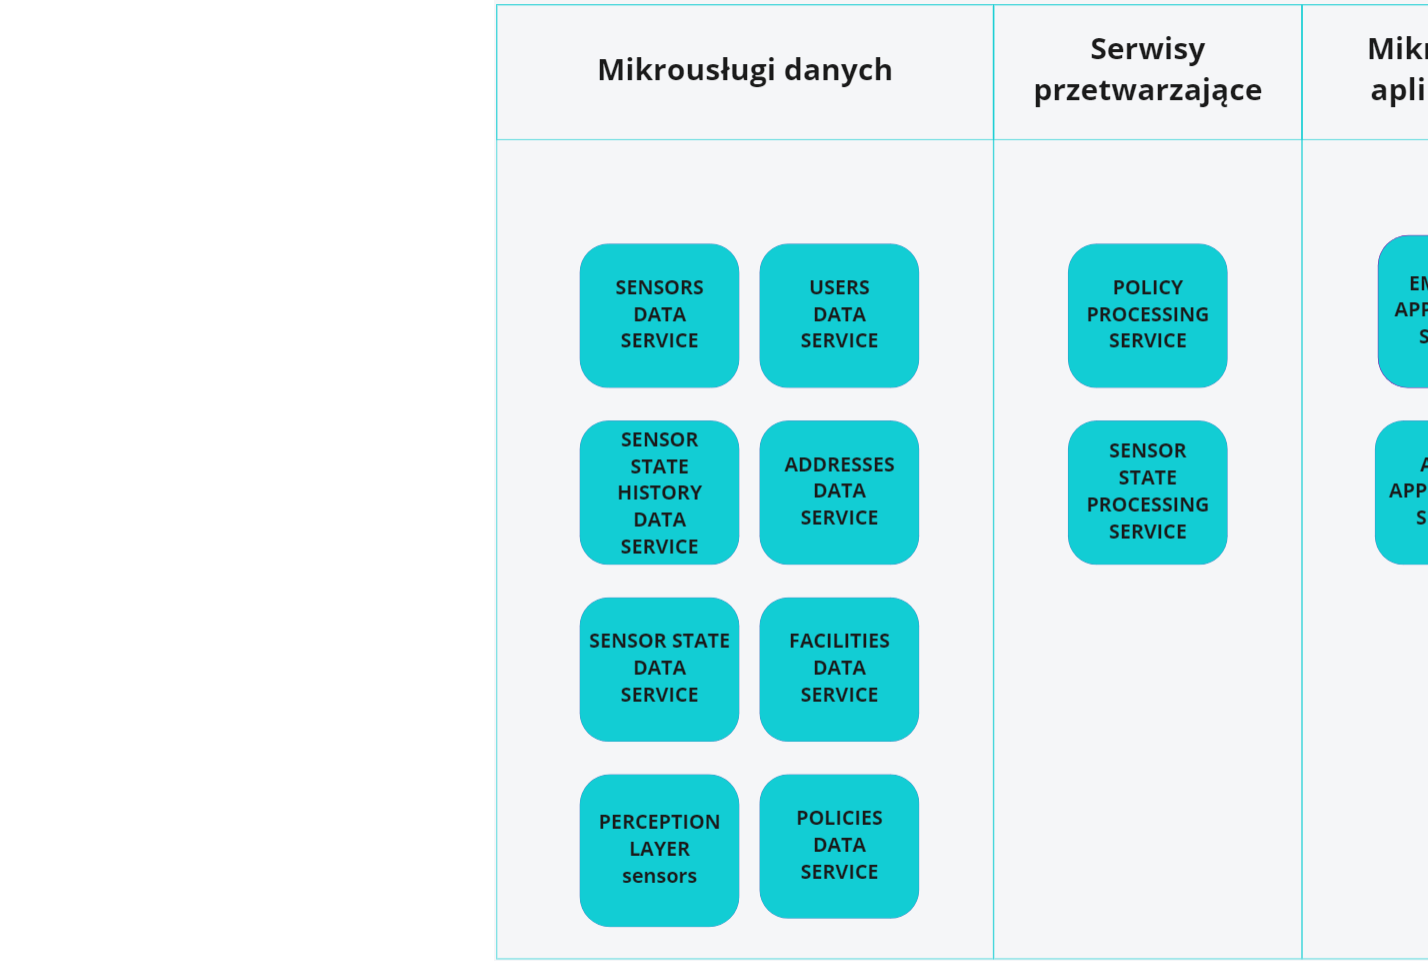
\includegraphics[width=1\textwidth]{architektura.jpg} % dodanie grafiki "thesis.jpg"
    \caption{Architektura systemu} % opis obrazka
    \label{fig:architektura-systemu} % labelka do figury, dzieki ktorej mozna sie pozniej do obrazka odnosic
\end{figure}

Na całość składają się serwisy opisane w tabeli \ref{tab:mikrouslugi-danych}.

\begin{table}[!ht]
    \caption{Mikrousługi danych}
    \label{tab:mikrouslugi-danych}
    \begin{tabularx}{1\textwidth} { 
        | >{\raggedright\arraybackslash}X        
        | >{\raggedleft\arraybackslash}X | }
        \hline
       Nazwa & Funkcja \\
       \hline
       Addresses data service & 
       Przechowuje adresy organizacji oraz poszczególnych budynków \\
       \hline
       Facilities data service &
       Przechowuje szczegółowe dane dotyczące budynków \\
       \hline
       Policies data service & 
       Przechowuje reguły określające oczekiwaną wartość mierzonych parametrów \\
       \hline
       Sensors data service &
       Przechowuje szczegółowe dane dotyczące wykorzystywanych czujników \\
       \hline
       Sensor state history data service &
       Przechowuje historyczne pomiary z poszczególnych czujników \\
       \hline
       Sensor state data service &
       Przesyła pomiary od czujników \\
       \hline
    \end{tabularx}
\end{table}

Poza mikrousługami danych aplikacja posiada również serwisy przetwarzające dane:

\begin{table}[!ht]
    \caption{Serwisy przetwarzające}
    \label{tab:serwisy-przetwarzajace}
    \begin{tabularx}{1\textwidth} { 
        | >{\raggedright\arraybackslash}X        
        | >{\raggedleft\arraybackslash}X | }
        \hline
       Nazwa & Funkcja \\
       \hline
       Sensor state processing service & 
       Otrzymuje dane z czujników. Zajmuje się ich prawidłowym zapisaniem, po czym wysyła 
       je dalej do serwisu sprawdzającego zgodność wyników rzeczywistych z oczekiwanymi \\
       \hline
       Policy processing service &
       Przetwarza dane z czujników. Porównuje pomiary rzeczywiste z oczekiwanymi, które 
       zostały określone w regułach \\
       \hline
    \end{tabularx}
\end{table}

Na system składają się także mikrousługi aplikacyjne:

\begin{table}[!ht]
    \caption{Mikrousługi aplikacyjne}
    \label{tab:mikrouslugi-aplikacyjne}
    \begin{tabularx}{1\textwidth} { 
        | >{\raggedright\arraybackslash}X        
        | >{\raggedleft\arraybackslash}X | }
        \hline
       Nazwa & Funkcja \\
       \hline
       Employee application service & 
       Usługa aplikacyjna dla aplikacji pracowników. Oferuje styki umożliwiające 
       zarządzanie kontem, tworzenie własnych reguł dla pomieszczeń przypisanych do 
       konkretnego użytkownika oraz sprawdzanie ich aktualnego stanu \\
       \hline
       Admin application service &
       Usługa aplikacyjna dla aplikacji administratorów. Oferuje wszystkie styki 
       udostępniane pracownikom, a ponadto styki umożliwiające zarządzanie informacjami 
       dotyczącymi organizacji, budynków, pomieszczeń i czujników \\
       \hline
    \end{tabularx}
\end{table}

Ostatnimi elementami systemu są aplikacje dla poszczególnych ról użytkowników:

\begin{table}[!ht]
    \caption{Aplikacje użytkowników}
    \label{tab:aplikacje-uzytkownikow}
    \begin{tabularx}{1\textwidth} { 
        | >{\raggedright\arraybackslash}X        
        | >{\raggedleft\arraybackslash}X | }
        \hline
       Nazwa & Funkcja \\
       \hline
       Employee application & 
       Oferuje graficzny interfejs do interakcji z usługą aplikacyjną pracowników \\
       \hline
       Admin application &
       Oferuje graficzny interfejs do interakcji z usługą aplikacyjną administratorów \\
       \hline
    \end{tabularx}
\end{table}

\section{Przechowywanie danych}

Poszczególne mikroserwisy odwołują się do różnych źródeł danych w celu uzyskania 
wymaganych informacji. W tej pracy wykorzystano dwa różne sposoby przechowywania 
informacji:

\begin{itemize} % lista nienumerowana
    \item Relacyjna baza danych MySQL
    \item Baza danych szeregów czasowych InfluxDB
\end{itemize}

\subsection{MySQL}

Relacyjna baza danych MySQL oferuje szybki, wielowątkowy serwer bazodanowy w oparciu 
o język SQL (ang. Structured Query Language). Została ona wybrana ze względu na to, że 
jest produktem typu open-source dostępną na licencji GNU (ang. general public license). 

Dobrą praktyką, którą warto mieć na uwadze podczas tworzenia systemu opartego na 
architekturze mikroserwisowej, jest zapewnienie dostępu do danego zbioru danych tylko 
jednemu mikroserwisowi, który następnie może je udostępniać przy pomocy odpowiednio 
skonfigurowanego API (Richardson, 2021). Takie podejście umożliwia zachowanie luźnego 
sprzężenia między serwisami. W konsekwencji należy utworzyć oddzielne zbiory 
danych, zwane schematami, które mogą być zarządzane przez pojedynczy mikroserwis.

W ramach utworzonego serwera bazodanowego zostały wdrożone następujące schematy:

\begin{table}[!ht]
    \caption{Utworzone schematy bazodanowe}
    \label{tab:schematy-bazodanowe}
    \begin{tabularx}{1\textwidth} { 
        | >{\raggedright\arraybackslash}X        
        | >{\raggedleft\arraybackslash}X | }
        \hline
       Nazwa schematu & Funkcja \\
       \hline
       Addresses (adresy) & 
       Przechowuje dane dotyczące adresów \\
       \hline
       Facilities (organizacje) &
       Przechowuje dane dotyczące organizacji oraz budynków \\
       \hline
       Identity (użytkownicy) &
       Przechowuje dane użytkowników \\
       \hline
       Policies (reguły) &
       Przechowuje dane dotyczące reguł określających oczekiwaną wartość mierzonych 
       parametrów \\
       \hline
       Sensors (sensory) & 
       Przechowuje dane dotyczące wykorzystywanych sensorów \\
       \hline
    \end{tabularx}
\end{table}

\subsubsection{Schemat adresów}

Schemat adresów składa się z następujących encji:

\begin{table}[!ht]
    \caption{Encje w schemacie adresów}
    \label{tab:encje-adresow}
    \begin{tabularx}{1\textwidth} { 
        | >{\raggedright\arraybackslash}X        
        | >{\raggedleft\arraybackslash}X | }
        \hline
       Nazwa encji & Przechowywane dane \\
       \hline
       Addresses & 
       Encja główna, zawiera odwołania do kraju, miasta, kodu pocztowego, numeru ulicy 
       oraz numeru budynku \\
       \hline
       Cities & Miasto \\
       \hline
       Countries & Kraj \\
       \hline
       Postal codes & Kod pocztowy \\
       \hline
       Streets & Ulica \\
       \hline
       Street numbers & Numer budynku \\
       \hline
    \end{tabularx}
\end{table}

Związki między poszczególnymi encjami zostały opisane w tabeli 10.


\begin{table}[!ht]
    \caption{Związki między encjami w schemacie adresów}
    \label{tab:zwiazki-adresy}
\begin{tabularx}{1\textwidth} { 
        | >{\arraybackslash}X    
        | >{\arraybackslash}X
        | >{\arraybackslash}X     
        | >{\arraybackslash}X | }
        \hline
    \multicolumn{2}{|c|}{Relacja} & Typ związku & Opis \\
    \hline
    Addresses & Countries & 1:N & 
    Każdy kraj może występować w wielu adresach \\
    \hline
    Addresses & Cities & 1:N & 
    Każde miasto może występować w wielu adresach \\
    \hline
    Addresses & Postal codes & 1:N 
    & Każdy kod pocztowy może występować w wielu adresach \\
    \hline
    Addresses & Strees & 1:N & 
    Każda ulica może występować w wielu adresach \\
    \hline
    Addresses & Street numbers & 1:N & 
    Każdy numer budynku może występować w wielu adresach \\
    \hline
    \end{tabularx}
\end{table}

\subsubsection{Schemat organizacji}

Schemat organizacji składa się z następujących encji:

\begin{table}[!ht]
    \caption{Encje w schemacie organizacji}
    \label{tab:encje-organizacji}
    \begin{tabularx}{1\textwidth} { 
        | >{\raggedright\arraybackslash}X        
        | >{\raggedleft\arraybackslash}X | }
        \hline
       Nazwa encji & Przechowywane dane \\
       \hline
       Affiliates & 
       Oddziały danej organizacji \\
       \hline
       Rooms & Pomieszczenia w oddziałach \\
       \hline
       Organizations & Organizacje \\
       \hline
    \end{tabularx}
\end{table}

Związki między poszczególnymi encjami zostały opisane w tabeli \ref{tab:zwiazki-organizacje}.


\begin{table}[!ht]
    \caption{Związki między encjami w schemacie organizacji}
    \label{tab:zwiazki-organizacje}
\begin{tabularx}{1\textwidth} { 
        | >{\arraybackslash}X    
        | >{\arraybackslash}X
        | >{\arraybackslash}X     
        | >{\arraybackslash}X | }
        \hline
    \multicolumn{2}{|c|}{Relacja} & Typ związku & Opis \\
    \hline
    Organizations & Affiliates & 1:N & 
    Każdy organizacja może posiadać wiele oddziałów \\
    \hline
    Affiliates & Rooms & 1:N & 
    Każdy oddział może posiadać wiele pomieszczeń \\
    \hline
    \end{tabularx}
\end{table}

\subsubsection{Schemat reguł}

Schemat reguł składa się z następujących encji:

\begin{table}[!ht]
    \caption{Encje w schemacie reguł}
    \label{tab:encje-regul}
    \begin{tabularx}{1\textwidth} { 
        | >{\raggedright\arraybackslash}X        
        | >{\raggedleft\arraybackslash}X | }
        \hline
       Nazwa encji & Przechowywane dane \\
       \hline
       Room policies & 
       Encja główna, zawiera odwołania do kategorii oraz oczekiwanych warunków. Przechowuje 
       okres obowiązywania danej reguły \\
       \hline
       Room policy categories & Kategorie reguł \\
       \hline
       Expected room conditions & Oczekiwane warunki w pomieszczeniu \\
       \hline
    \end{tabularx}
\end{table}

Związki między poszczególnymi encjami zostały opisane w tabeli \ref{tab:zwiazki-reguly}.


\begin{table}[!ht]
    \caption{Związki między encjami w schemacie reguł}
    \label{tab:zwiazki-reguly}
\begin{tabularx}{1\textwidth} { 
        | >{\arraybackslash}X    
        | >{\arraybackslash}X
        | >{\arraybackslash}X     
        | >{\arraybackslash}X | }
        \hline
    \multicolumn{2}{|c|}{Relacja} & Typ związku & Opis \\
    \hline
    Room policies & Room policy categories & 1:N & 
    Każda kategoria może być przypisana wielu regułom \\
    \hline
    Room policies & Expected room conditions & 1:N & 
    Ten sam zbiór oczekiwanych warunków może być przypisany do wielu reguł \\
    \hline
    \end{tabularx}
\end{table}

\subsubsection{Schemat sensorów}

Schemat sensorów składa się z następujących encji:

\begin{table}[!ht]
    \caption{Encje w schemacie sensorów}
    \label{tab:encje-sensorow}
    \begin{tabularx}{1\textwidth} { 
        | >{\raggedright\arraybackslash}X        
        | >{\raggedleft\arraybackslash}X | }
        \hline
       Nazwa encji & Przechowywane dane \\
       \hline
       Sensors & Szczegóły dotyczące danego sensora \\
       Sensor models & Model sensora \\
       Producers & Producent sensorów \\
       \hline
    \end{tabularx}
\end{table}

Związki między poszczególnymi encjami zostały opisane w tabeli \ref{tab:zwiazki-sensory}.

\begin{table}[!ht]
    \caption{Związki między encjami w schemacie sensorów}
    \label{tab:zwiazki-sensory}
\begin{tabularx}{1\textwidth} { 
        | >{\arraybackslash}X    
        | >{\arraybackslash}X
        | >{\arraybackslash}X     
        | >{\arraybackslash}X | }
        \hline
    \multicolumn{2}{|c|}{Relacja} & Typ związku & Opis \\
    \hline
    Sensor models & Producers & 1:N & 
    Każdy producent może oferować wiele modeli sensorów \\
    \hline
    Sensor models & Sensors & 1:N & 
    Każdy model może być wypordukowany wielokrotnie \\
    \hline
    \end{tabularx}
\end{table}

\subsubsection{Schemat użytkowników}

Schemat użytkowników został oparty na schemacie oferowanym przez Microsoft 
\parencite{vickers:2021an} i składa się z następujących encji:

\begin{table}[!ht]
    \caption{Encje w schemacie użytkowników}
    \label{tab:encje-uzytkownicy}
    \begin{tabularx}{1\textwidth} { 
        | >{\raggedright\arraybackslash}X        
        | >{\raggedleft\arraybackslash}X | }
        \hline
       Nazwa encji & Przechowywane dane \\
       \hline
       Asnetusers & Reprezentuje użytkownika \\
       \hline
       Aspnetroles & Reprezentuje rolę użytkownika w systemie \\
       \hline
       Aspnetuserlogins & Łączy użytkownika z loginem \\
       \hline
       Aspnetusertokens & Reprezentuje token uwierzytelniający dla użytkownika \\
       \hline
       Aspnetuserclaims & Reprezentuje prawa, które posiada użytkownik \\
       \hline
       Aspnetroleclaims & Reprezentuje prawa gwarantowane dla wszystkich użytkowników
       pełniących daną rolę \\
       \hline
       Aspnetuserroles & Łączy użytkowników z poszczególnymi rolami \\
       \hline
    \end{tabularx}
\end{table}

Związki między poszczególnymi encjami zostały opisane w tabeli \ref{tab:zwiazki-uzytkownicy}.

\begin{table}[!ht]
    \caption{Związki między encjami w schemacie użytkowników}
    \label{tab:zwiazki-uzytkownicy}
\begin{tabularx}{1\textwidth} { 
        | >{\arraybackslash}X    
        | >{\arraybackslash}X
        | >{\arraybackslash}X     
        | >{\arraybackslash}X | }
        \hline
    \multicolumn{2}{|c|}{Relacja} & Typ związku & Opis \\
    \hline
    Aspnetusers & Aspnetuserlogins & 1:N & 
    Każdemu użytkownikowi może być przypisanych wiele loginów \\
    \hline
    Aspnetusers & Aspnetusertokens & 1:N & 
    Każdemu użytkownikowi może być przypisanych wiele tokenów \\
    \hline
    Aspnetusers & Aspnetuserroles & 1:N &
    Każdy użytkownik może pełnić wiele ról \\
    \hline
    Aspnetusers & Aspnetuserclaims & 1:N &
    Każdy użytkownik może posiadać wiele praw \\
    \hline
    Aspnetroles & Aspnetroleclaims & 1:N &
    Każdej roli może być przypisanych wiele praw \\
    \hline
    Aspnetroles & Aspnetuserroles & 1:N &
    Każda rola może być pełniona przez wielu użytkowników \\
    \hline
    \end{tabularx}
\end{table}

\subsection{InfluxDB}

InfluxDB jest bazą danych szeregów czasowych służącą do przechowywania metryk 
i szeregów czasowych. Umożliwia efektywne przechowywanie miliardów rekordów danych 
dzięki stosowaniu kompresji danych, oferuje także język zapytań pozwalający 
przeprowadzać kompleksowe analizy uzyskanych danych. Dodatkową funkcjonalnością 
wyróżniającą tą bazę od standardowych relacyjnych baz danych jest możliwość 
zdefiniowania czasu, po którym rekordy będą usuwane. Można w ten sposób określić na 
przykład, że baza powinna przechowywać tylko rekordy z ostatniego miesiąca.

W tej pracy inżynierskiej baza danych szeregów czasowych została wykorzystana do 
przechowywania danych zbieranych z czujników temperatury oraz natężenia światła. 
Przychodzące informacje są zapisywane w kolejnych rekordach, które zawierają 
następujące parametry:

\begin{table}[!ht]
    \caption{Parametry pojedynczego rekordu przechowującego pomiar}
    \label{tab:parametry-pomiaru}
    \begin{tabularx}{1\textwidth} { 
        | >{\raggedright\arraybackslash}X 
        | >{\raggedleft\arraybackslash}X | }
        \hline
       Parametr & Znaczenie \\
       \hline
       time & Czas otrzymania danych \\
       \hline
       field & Rodzaj danych \\
       \hline
       value & Zmierzona wartość \\
       \hline
    \end{tabularx}
\end{table}


{Komunikacja między serwisami}
\subsection{Broker wiadomości}
\section
Aby mikroserwisy mogły działać poprawnie, potrzebują wymieniać ze sobą informacje 
w sposób szybki i niezawodny. W przypadku komunikacji nie wymagającej żadnej interakcji 
z użytkownikiem, jednym z rozwiązań jest wykorzystanie brokera wiadomości, który pełni 
rolę pośrednika przekazującego wiadomości między serwisami. Do grona takich narzędzi 
należy RabbitMQ. Spośród konkurencyjnych rozwiązań wyróżnia się tym, że jest to 
narzędzie typu open source, ponadto cechuje się małymi wymaganiami sprzętowymi oraz 
łatwością wdrażania w chmurze. 

RabbitMQ wspiera różne protokoły do przekazywania wiadomości, jednak domyślnie 
wykorzystuje protokół AMQP 0-9-1 (ang. advanced message queuing protocol). Uogólniony 
schemat, na którym opiera się protokoł, został przedstawiony na rysunku \ref{fig:schemat-amqp}.

\begin{figure}[h]
    \centering
    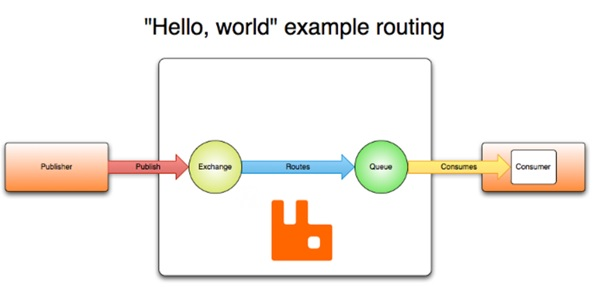
\includegraphics[width=1\textwidth]{amqp_schema.jpg}
    \caption{Schemat protokołu AMQP 0-9-1. Źródło: \href{https://www.rabbitmq.com/tutorials/amqp-concepts.html}{Schemat AMQP}}
    \label{fig:schemat-amqp}
\end{figure}

Wydawcy wiadomości (ang. publisher) publikują wiadomości do pośrednika, który następnie 
przekuje je do odpowiednich konsumentów (ang. consumer). Ponieważ jest to protokół 
sieciowy, to wydawcy, konsumenci oraz pośrednicy mogą być uruchomieni na różnych 
maszynach. Pośrednik RabbitMq dysponuje następującymi cechami:

\begin{itemize} % lista nienumerowana
    \item Wiadomości są publikowane na giełdy (ang. exchange)
    \item Giełdy mogą być połączone z wieloma kolejkami (ang. queue)
    \item Zależnie od zastosowanej polityki kopia wiadomości może być przekazana do 
    każdej powiązanej kolejki lub tylko podzbiorowi kolejek
    \item Kolejka po otrzymaniu wiadomości od giełdy przesyła ją do konsumentów
\end{itemize}

Przesyłanie informacji przez sieć wiąże się z ryzykiem tego, że dane nie zostaną 
dostarczone. Wobec tego protokół zapewnia funkcjonalność, zwaną potwierdzeniem 
wiadomości (ang. message acknowledgements), która gwarantuje otrzymanie wiadomości 
przez konsumentów. Działa ona w ten sposób, że wiadomość jest usuwana z kolejki tylko 
wtedy, gdy uzyska potwierdzenie jej otrzymania od zainteresowanych usług.

Giełdy po otrzymaniu wiadomości od wydawców mogą ją rozesłać do zera lub większej 
liczby kolejek. Używany algorytm routingu zależy od typu wymiany i reguł nazywanych 
powiązaniami (ang. bindings). Pośrednicy korzystający z protokołu AMQP 0-9-1 zapewniają 
cztery typy wymiany:

\begin{itemize} % lista nienumerowana
    \item Wymiana bezpośrednia (ang direct exchange) - dostarcza wiadomości do kolejek 
    na podstawie klucza routingu. Jest idealna do wiadomości typu unicast 
    (chociaż może być także używana do wiadomości typu multicast)
    \item Wymiana do wszystkich (fanout exchange) - kieruje komunikaty do wszystkich 
    kolejek, które są z nią powiązane, a klucz routingu jest ignorowany. Jeśli do 
    giełdy dowiązanych jest N kolejek, to po publikacji wiadomości przez wydawcę 
    dotrze ona do wszystkich N kolejek. Jest idealna do rozsyłania wiadomości do 
    wszystkich usług
    \item Wymiana tematyczna (ang. topic exchange) - kierują wiadomości do jednej lub 
    wielu kolejek na podstawie dopasowania klucza routingu oraz wzorca użytego do 
    powiązania kolejki z giełdą. Jest często używana do implementacji różnych odmian 
    wzorca publish/subscribe. Typowo używa się jej dla wiadomości typu multicast. 
    Warto ją rozważyć w przypadku, gdy należy dostarczyć wiadomość do wielu 
    konsumentów, które selektywnie wybierają rodzaj wiadomości, które chcą otrzymywać
    \item Wymiana nagłówków (ang. headers exchange) - przeznaczona do routingu na 
    podstawie wielu atrybutów, które łatwiej można wyrazić w postaci nagłówków 
    wiadomości niż klucza routingu, który jest ignorowany. Wiadomość uważana jest za 
    zgodną i rozsyłana dalej, jeśli wartość nagłówka jest równa wartości określonej 
    podczas wiązania
\end{itemize}

AMQP 0-9-1 jest protokołem poziomu aplikacji, który używa protokołu TCP do niezawodnego 
przesyłania wiadomości. Połączenia (ang. connections) korzystają z metod 
uwierzytelnienia i mogą być chronione za pomocą protokołu TLS. Ze względu na dodatkowe 
środki zapewniające niezawodność zaleca się, aby połączenia między klientem 
a pośrednikiem były ustanawiane na dłuższy okres czasu. W przypadku gdy klient 
potrzebuje nawiązać wiele połączeń, może skorzystać z kanałów (ang. 
channels), o których można myśleć jako lekkich połączeniach dzielących jedno 
połączenie TCP. Każda operacja przeprowadzana przez klienta odbywa się z użyciem 
kanału, a komunikacja na różnych kanałach jest od siebie całkowicie odseparowana. 
Z tego względu każda metoda zawiera identyfikator kanału dla rozróżnienia, przez 
który kanał należy wysłać wiadomość.

\subsubsection{MassTransit}

Przy tworzeniu systemu została wykorzystana szyna danych o nazwie MassTransit 
przeznaczona dla aplikacji napisanych we framework'u .NET Core. Zapewnia ona poziom 
abstrakcji umożliwiający wykorzystanie wielu różnych pośredników wiadomości, w 
tym RabbitMQ. Spośród wielu swoich zalet, szyna zapewnia:

\begin{itemize} % lista nienumerowana
    \item Równoczesne, asynchroniczne przetwarzanie wiadomości dla zwiększenia 
    przepustowości
    \item Zarządzanie połączeniem. Jeśli dany mikroserwis zostanie rozłączony 
    z pośrednikiem wiadomości, MassTransit spróbuje połączyć się ponownie oraz 
    przywrócić dotychczasowe giełdy, kolejki, a także połączenia między nimi
    \item Serializacja danych. Pośrednik wiadomości RabbitMq przesyła wiadomości 
    w postaci bajtów. Aby za jego pomocą przesłać obiekty specyficzne dla języka 
    C\#, trzeba zapisać je w odpowiednim formacie, w procesie zwanym serializacją. 
    MassTransit implementuje narzędzia do serializacji obiektów
    \item Testy jednostkowe. MassTransit zawiera implementację przygotowaną specjalnie 
    do testów w taki sposób, by testy nie były zależne od reszty infrakstruktury 
    systemu. Przykładem jest poniższa metoda:
\end{itemize}

\begin{lstlisting}
    internal static async Task PublishAndWaitToBeConsumed<T>(T @event, InMemoryTestHarness testHarness)
    {
        var messageIdentifier = await PublishMessage(@event, testHarness);

        var messageHasBeenConsumed = await testHarness.Consumed.Any(x => x.Context.MessageId == messageIdentifier);
        messageHasBeenConsumed.Should().BeTrue();

        var message = await testHarness!.Consumed.SelectAsync(x => x.Context.MessageId == messageIdentifier).First();
        message.Exception.Should().BeNull("Message has been consumed without any errors");
    }
    \end{lstlisting}

Metoda publikuje testową wiadomość, po czym sprawdza, czy została prawidłowo 
przetworzona. 

Dzięki zastosowaniu szyny danych tworzenie konsumentów oraz publikowanie wiadomości 
staje się dużo łatwiejsze. Aby utworzyć nowego konsumenta, wystarczy jedynie utworzyć 
nową klasę implementującą interfejs IConsumer<T>, gdzie T jest oczekiwanym typem 
wiadomości. Klasa musi zawierać implementację metody 
Consume(ConsumeContext<MeasurementSentEvent> context), która zawiera logikę 
przetwarzania wiadomości. Przykładem jest poniższa metoda:

\begin{lstlisting}
    public async Task Consume(ConsumeContext<MeasurementSentEvent> context)
    {
        var policiesEvaluationResultEvent = await _evaluatePoliciesCommand.Handle(context.Message);

        await _eventPublisher.Publish(policiesEvaluationResultEvent);
        _logger.LogInformation($"PoliciesEvaluationResultEvent sent from PolicyNode. Message: {policiesEvaluationResultEvent.Message}");
    }

    \end{lstlisting}
    
Zapisuje ona w logach szczegóły dotyczące przychodzącej wiadomości, przetwarza 
otrzymane wartości, po czym publikuje nową wiadomość o innym typie, której konsument 
znajduje się w innym mikroserwisie.

\subsubsection{Połączenie serwisów z brokerem wiadomości}

Utworzone w ramach pracy mikroserwisy łączą się z brokerem wiadomości i w ten sposób wymieniają między
sobą dane. Mogą one być połączone w różny sposób, zależnie od oczekiwanego rezultatu. Dwa główne
przypadki zostały przedstawione na rysunku \ref{fig:rabbitmq-polaczenie}.

\begin{figure}[h]
    \centering
    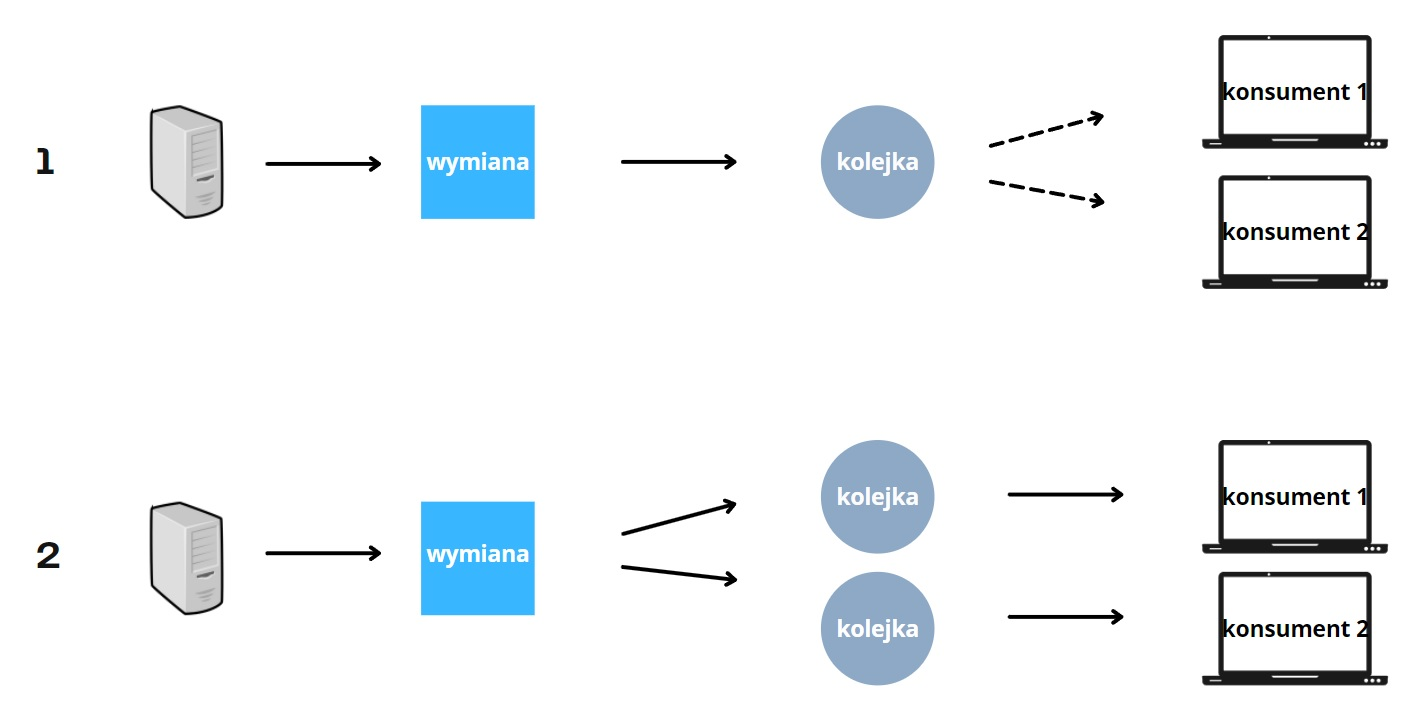
\includegraphics[width=1\textwidth]{rabbitmq_schema.jpg}
    \caption{Rodzaje połączenia z brokerem wiadomości}
    \label{fig:rabbitmq-polaczenie}
\end{figure}

\begin{enumerate} % lista numerowana
    \item W pierwszym przypadku celem jest wysłanie wiadomości tylko do jednego konsumenta. Jedną
    z występujących sytuacji jest przetwarzanie otrzymanych z czujników pomiarów przez Sensor State
    Processing Service. Wykonanie tej samej operacji przez kilka instancji tego serwisu byłoby stratą
    dostępnych zasobów. Aby osiągnąć ten efekt, wszystkie instancje tego serwisu powinny być dołączone 
    do jednej kolejki. Wtedy kolejka wysyła przychodzące pomiary tylko do wybranej przez siebie instancji.
    Wybór odbywa się za pomocą mechanizmu szeregowania procesów Round-robin.
    \item W drugim przypadku celem jest wysłanie wiadomości do wielu konsumentów. Jedną z występujących
    sytuacji jest wysłanie wyniku przetwarzania pomiarów do wszystkich pracowników oraz administratorów
    posiadających uprawnienia do jego wyświetlenia. Aby osiągnąć ten efekt, każda instancja serwisów
    otrzymujących wynik (w tym wypadku są to Admin Application Service oraz Employee Application Service)
    powinna być dołączona do osobnej kolejki, z których wszystkie dołączone są do tej samej giełdy
    publikującej wiadomości. W ten sposób kopia wysłanej przez wydawcę wiadomości zostanie dostarczona
    do każdej instancji.
\end{enumerate}

\subsection{Styki}

Mikroserwisy mogą komunikować się między sobą przy użyciu oferowanych przez nie 
styków (ang. Application Programming Interface). Definiują one kontrakty 
określające informacje wymagane przy wysyłaniu żądania oraz zbiór danych zwracany 
w odpowiedzi.

Mikrousługi aplikacyjne oraz mikrousługi danych oferują styki zwracające jasno 
zdefiniowany zbiór danych. Zostały one szczegółowo opisane w poniższych podrozdziałach. 
Każdy ze styków zawiera:

\begin{itemize} % lista nienumerowana
    \item Krótki opis funkcjonalności
    \item Wykorzystywany czasownik protokołu http. Jeden z GET, POST, UPDATE, DELETE
    \item wymagane parametry wejściowe
    \item numer statusu oraz typ zwracanego obiektu
\end{itemize}

\subsubsection{Styk mikrousługi danych adresów}

\begin{table}[!ht]
    \caption{Endpoint 1}
    \label{tab:adresy-endpoint1}
\begin{tabularx}{1\textwidth} { 
        | c    
        | c
        | X | }
        \hline
    \textbf{Ścieżka} & 
    \multicolumn{2}{c|}{GET /addresses-api/addresses/{addressId}} \\
    \hline
    \textbf{Opis} & 
    \multicolumn{2}{c|}{\makecell{Zwraca informacje na temat adresu o danym identyfikatorze}} \\    \hline
    \textbf{Odpowiedź} &
    \textbf{Kod odpowiedzi} &
    \textbf{Schemat} \\
    \hline
    {} & 200 & AddressDtoJsonApiDocument \\
    \hline
    {} & 404 & JsonApiError \\
    \hline
    \end{tabularx}
\end{table}

\begin{table}[!ht]
    \caption{Endpoint 1}
    \label{tab:adresy-endpoint2}
\begin{tabularx}{1\textwidth} { 
        | c    
        | c
        | X | }
        \hline
    \textbf{Ścieżka} & 
    \multicolumn{2}{c|}{POST /addresses-api/addresses} \\
    \hline
    \textbf{Opis} & 
    \multicolumn{2}{c|}{\makecell{Tworzy nowy adres o parametrach podanych \\ w modelu AddNewAddressCommand}} \\    \hline
    \textbf{Odpowiedź} &
    \textbf{Kod odpowiedzi} &
    \textbf{Schemat} \\
    \hline
    {} & 201 & AddressDtoJsonApiDocument \\
    \hline
    {} & 400 & JsonApiError \\
    \hline
    \end{tabularx}
\end{table}

\begin{table}[!ht]
    \caption{Endpoint 1}
    \label{tab:adresy-endpoint3}
\begin{tabularx}{1\textwidth} { 
        | c    
        | c
        | X | }
        \hline
    \textbf{Ścieżka} & 
    \multicolumn{2}{c|}{GET /addresses-api/cities/{cityId}} \\
    \hline
    \textbf{Opis} & 
    \multicolumn{2}{c|}{\makecell{Zwraca informacje na temat miasta o danym identyfikatorze}} \\    \hline
    \textbf{Odpowiedź} &
    \textbf{Kod odpowiedzi} &
    \textbf{Schemat} \\
    \hline
    {} & 200 & CityDtoJsonApiDocument \\
    \hline
    {} & 404 & JsonApiError \\
    \hline
    \end{tabularx}
\end{table}

\begin{table}[!ht]
    \caption{Endpoint 1}
    \label{tab:adresy-endpoint4}
\begin{tabularx}{1\textwidth} { 
        | c    
        | c
        | X | }
        \hline
    \textbf{Ścieżka} & 
    \multicolumn{2}{c|}{GET /addresses-api/countries/{countryId}} \\
    \hline
    \textbf{Opis} & 
    \multicolumn{2}{c|}{\makecell{Zwraca informacje na temat kraju o danym identyfikatorze}} \\    \hline
    \textbf{Odpowiedź} &
    \textbf{Kod odpowiedzi} &
    \textbf{Schemat} \\
    \hline
    {} & 200 & CountryDtoJsonApiDocument \\
    \hline
    {} & 404 & JsonApiError \\
    \hline
    \end{tabularx}
\end{table}

\begin{table}[!ht]
    \caption{Endpoint 1}
    \label{tab:adresy-endpoint5}
\begin{tabularx}{1\textwidth} { 
        | c    
        | c
        | X | }
        \hline
    \textbf{Ścieżka} & 
    \multicolumn{2}{c|}{GET /addresses-api/postal-codes/{postalCodeId}} \\
    \hline
    \textbf{Opis} & 
    \multicolumn{2}{c|}{\makecell{Zwraca informacje na temat kodu pocztowego o danym identyfikatorze}} \\    \hline
    \textbf{Odpowiedź} &
    \textbf{Kod odpowiedzi} &
    \textbf{Schemat} \\
    \hline
    {} & 200 & PostalCodeDtoJsonApiDocument \\
    \hline
    {} & 404 & JsonApiError \\
    \hline
    \end{tabularx}
\end{table}

\subsubsection{Styk mikrousługi danych organizacji}

\begin{table}[!ht]
    \caption{Endpoint 1}
    \label{tab:organizacje-endpoint1}
\begin{tabularx}{1\textwidth} { 
        | c    
        | c
        | X | }
        \hline
    \textbf{Ścieżka} & 
    \multicolumn{2}{c|}{POST /facilities-api/affiliates} \\
    \hline
    \textbf{Opis} & 
    \multicolumn{2}{c|}{\makecell{Tworzy nowy oddział o parametrach podanych \\w modelu AddNewAffiliateCommand}} \\    \hline
    \textbf{Odpowiedź} &
    \textbf{Kod odpowiedzi} &
    \textbf{Schemat} \\
    \hline
    {} & 201 & AffiliateDtoJsonApiDocument \\
    \hline
    {} & 400 & JsonApiError \\
    \hline
    {} & 409 & JsonApiError \\
    \hline
    \end{tabularx}
\end{table}

\begin{table}[!ht]
    \caption{Endpoint 1}
    \label{tab:organizacje-endpoint2}
\begin{tabularx}{1\textwidth} { 
        | c    
        | c
        | X | }
        \hline
    \textbf{Ścieżka} & 
    \multicolumn{2}{c|}{GET /facilities-api/affiliates} \\
    \hline
    \textbf{Opis} & 
    \multicolumn{2}{c|}{\makecell{Zwraca informacje na temat wszystkich oddziałów}} \\    \hline
    \textbf{Odpowiedź} &
    \textbf{Kod odpowiedzi} &
    \textbf{Schemat} \\
    \hline
    {} & 200 & AffiliateDtoListJsonApiDocument \\
    \hline
    \end{tabularx}
\end{table}

\begin{table}[!ht]
    \caption{Endpoint 1}
    \label{tab:organizacje-endpoint3}
\begin{tabularx}{1\textwidth} { 
        | c    
        | c
        | X | }
        \hline
    \textbf{Ścieżka} & 
    \multicolumn{2}{c|}{GET /facilities-api/affiliates/{affiliateId}} \\
    \hline
    \textbf{Opis} & 
    \multicolumn{2}{c|}{\makecell{Zwraca informacje na temat oddziału o danym identyfikatorze}} \\    \hline
    \textbf{Odpowiedź} &
    \textbf{Kod odpowiedzi} &
    \textbf{Schemat} \\
    \hline
    {} & 200 & AffiliateDtoJsonApiDocument \\
    \hline
    {} & 404 & JsonApiError \\
    \hline
    \end{tabularx}
\end{table}

\begin{table}[!ht]
    \caption{Endpoint 1}
    \label{tab:organizacje-endpoint4}
\begin{tabularx}{1\textwidth} { 
        | c    
        | c
        | X | }
        \hline
    \textbf{Ścieżka} & 
    \multicolumn{2}{c|}{DELETE /facilities-api/affiliates/{affiliateId}} \\
    \hline
    \textbf{Opis} & 
    \multicolumn{2}{c|}{\makecell{Usuwa informacje na temat oddziału o danym identyfikatorze}} \\    \hline
    \textbf{Odpowiedź} &
    \textbf{Kod odpowiedzi} &
    \textbf{Schemat} \\
    \hline
    {} & 204 & Brak zawartości \\
    \hline
    {} & 404 & JsonApiError \\
    \hline
    \end{tabularx}
\end{table}

\begin{table}[!ht]
    \caption{Endpoint 1}
    \label{tab:organizacje-endpoint5}
\begin{tabularx}{1\textwidth} { 
        | c    
        | c
        | X | }
        \hline
    \textbf{Ścieżka} & 
    \multicolumn{2}{c|}{POST /facilities-api/organizations} \\
    \hline
    \textbf{Opis} & 
    \multicolumn{2}{c|}{\makecell{Tworzy nową organizację o parametrach podanych \\w modelu AddNewOrganizationCommand}} \\    \hline
    \textbf{Odpowiedź} &
    \textbf{Kod odpowiedzi} &
    \textbf{Schemat} \\
    \hline
    {} & 201 & OrganizationDtoJsonApiDocument \\
    \hline
    {} & 400 & JsonApiError \\
    \hline
    {} & 409 & JsonApiError \\
    \hline
    \end{tabularx}
\end{table}

\begin{table}[!ht]
    \caption{Endpoint 1}
    \label{tab:organizacje-endpoint6}
\begin{tabularx}{1\textwidth} { 
        | c    
        | c
        | X | }
        \hline
    \textbf{Ścieżka} & 
    \multicolumn{2}{c|}{GET /facilities-api/organizations} \\
    \hline
    \textbf{Opis} & 
    \multicolumn{2}{c|}{\makecell{Zwraca informacje na temat wszystkich organizacji}} \\    \hline
    \textbf{Odpowiedź} &
    \textbf{Kod odpowiedzi} &
    \textbf{Schemat} \\
    \hline
    {} & 200 & OrganizationDtoListJsonApiDocument \\
    \hline
    \end{tabularx}
\end{table}

\begin{table}[!ht]
    \caption{Endpoint 1}
    \label{tab:organizacje-endpoint7}
\begin{tabularx}{1\textwidth} { 
        | c    
        | c
        | X | }
        \hline
    \textbf{Ścieżka} & 
    \multicolumn{2}{c|}{GET /facilities-api/organizations/{organizationId}} \\
    \hline
    \textbf{Opis} & 
    \multicolumn{2}{c|}{\makecell{Zwraca informacje na temat organizacji o danym identyfikatorze}} \\    \hline
    \textbf{Odpowiedź} &
    \textbf{Kod odpowiedzi} &
    \textbf{Schemat} \\
    \hline
    {} & 200 & OrganizationDtoJsonApiDocument \\
    \hline
    {} & 404 & JsonApiError \\
    \hline
    \end{tabularx}
\end{table}

\begin{table}[!ht]
    \caption{Endpoint 1}
    \label{tab:organizacje-endpoint8}
\begin{tabularx}{1\textwidth} { 
        | c    
        | c
        | X | }
        \hline
    \textbf{Ścieżka} & 
    \multicolumn{2}{c|}{DELETE /facilities-api/organizations/{organizationId}} \\
    \hline
    \textbf{Opis} & 
    \multicolumn{2}{c|}{\makecell{Usuwa informacje na temat organizacji o danym identyfikatorze}} \\    \hline
    \textbf{Odpowiedź} &
    \textbf{Kod odpowiedzi} &
    \textbf{Schemat} \\
    \hline
    {} & 204 & Brak zawartości \\
    \hline
    {} & 404 & JsonApiError \\
    \hline
    \end{tabularx}
\end{table}

\begin{table}[!ht]
    \caption{Endpoint 1}
    \label{tab:organizacje-endpoint9}
\begin{tabularx}{1\textwidth} { 
        | c    
        | c
        | X | }
        \hline
    \textbf{Ścieżka} & 
    \multicolumn{2}{c|}{POST /facilities-api/rooms} \\
    \hline
    \textbf{Opis} & 
    \multicolumn{2}{c|}{\makecell{Tworzy nowe pomieszczenie o parametrach podanych \\w modelu AddNewRoomCommand}} \\    \hline
    \textbf{Odpowiedź} &
    \textbf{Kod odpowiedzi} &
    \textbf{Schemat} \\
    \hline
    {} & 201 & RoomDtoJsonApiDocument \\
    \hline
    {} & 400 & JsonApiError \\
    \hline
    {} & 409 & JsonApiError \\
    \hline
    \end{tabularx}
\end{table}

\begin{table}[!ht]
    \caption{Endpoint 1}
    \label{tab:organizacje-endpoint10}
\begin{tabularx}{1\textwidth} { 
        | c    
        | c
        | X | }
        \hline
    \textbf{Ścieżka} & 
    \multicolumn{2}{c|}{GET /facilities-api/rooms/{roomId}} \\
    \hline
    \textbf{Opis} & 
    \multicolumn{2}{c|}{\makecell{Zwraca informacje na temat pomieszczenia o danym identyfikatorze}} \\    \hline
    \textbf{Odpowiedź} &
    \textbf{Kod odpowiedzi} &
    \textbf{Schemat} \\
    \hline
    {} & 200 & RoomDtoJsonApiDocument \\
    \hline
    {} & 404 & JsonApiError \\
    \hline
    \end{tabularx}
\end{table}

\begin{table}[!ht]
    \caption{Endpoint 1}
    \label{tab:organizacje-endpoint11}
\begin{tabularx}{1\textwidth} { 
        | c    
        | c
        | X | }
        \hline
    \textbf{Ścieżka} & 
    \multicolumn{2}{c|}{DELETE /facilities-api/rooms/{roomId}} \\
    \hline
    \textbf{Opis} & 
    \multicolumn{2}{c|}{\makecell{Usuwa informacje na temat pomieszczenia o danym identyfikatorze}} \\    \hline
    \textbf{Odpowiedź} &
    \textbf{Kod odpowiedzi} &
    \textbf{Schemat} \\
    \hline
    {} & 204 & Brak zawartości \\
    \hline
    {} & 404 & JsonApiError \\
    \hline
    \end{tabularx}
\end{table}

\subsubsection{Styk mikrousługi danych reguł}

\begin{table}[!ht]
    \caption{Endpoint 1}
    \label{tab:reguly-endpoint1}
\begin{tabularx}{1\textwidth} { 
        | c    
        | c
        | X | }
        \hline
    \textbf{Ścieżka} & 
    \multicolumn{2}{c|}{POST /policies-api/expected-room-conditions} \\
    \hline
    \textbf{Opis} & 
    \multicolumn{2}{c|}{\makecell{Tworzy nowy zestaw oczekiwanych wartości mierzonych\\parametrów określonych w modelu \\AddNewExpectedRoomConditionsCommand}} \\    \hline
    \textbf{Odpowiedź} &
    \textbf{Kod odpowiedzi} &
    \textbf{Schemat} \\
    \hline
    {} & 201 & OrganizationDtoJsonApiDocument \\
    \hline
    {} & 400 & JsonApiError \\
    \hline
    \end{tabularx}
\end{table}

\begin{table}[!ht]
    \caption{Endpoint 1}
    \label{tab:reguly-endpoint2}
\begin{tabularx}{1\textwidth} { 
        | c    
        | c
        | X | }
        \hline
    \textbf{Ścieżka} & 
    \multicolumn{2}{c|}{\makecell{GET /policies-api/expected-room-\\conditions/\{expectedRoomConditionsId\}}} \\
    \hline
    \textbf{Opis} & 
    \multicolumn{2}{c|}{\makecell{Zwraca informacje na temat zestawu oczekiwanych wartości\\mierzonych parametrów o danym identyfikatorze}} \\    \hline
    \textbf{Odpowiedź} &
    \textbf{Kod odpowiedzi} &
    \textbf{Schemat} \\
    \hline
    {} & 200 & RoomDtoJsonApiDocument \\
    \hline
    {} & 404 & JsonApiError \\
    \hline
    \end{tabularx}
\end{table}

\begin{table}[!ht]
    \caption{Endpoint 1}
    \label{tab:reguly-endpoint3}
\begin{tabularx}{1\textwidth} { 
        | c    
        | c
        | X | }
        \hline
    \textbf{Ścieżka} & 
    \multicolumn{2}{c|}{POST /policies-api/policies} \\
    \hline
    \textbf{Opis} & 
    \multicolumn{2}{c|}{\makecell{Tworzy nową regułę o parametrach określonych \\w modelu AddNewRoomPolicyCommand}} \\    \hline
    \textbf{Odpowiedź} &
    \textbf{Kod odpowiedzi} &
    \textbf{Schemat} \\
    \hline
    {} & 201 & RoomPolicyDtoJsonApiDocument \\
    \hline
    {} & 400 & JsonApiError \\
    \hline
    \end{tabularx}
\end{table}

\begin{table}[!ht]
    \caption{Endpoint 1}
    \label{tab:reguly-endpoint4}
\begin{tabularx}{1\textwidth} { 
        | c    
        | c
        | X | }
        \hline
    \textbf{Ścieżka} & 
    \multicolumn{2}{c|}{POST /policies-api/policies/past-policies} \\
    \hline
    \textbf{Opis} & 
    \multicolumn{2}{c|}{\makecell{Zwraca listę reguł poprzednio obowiązujących \\w pomieszczeniu określonym w modelu GetPastPoliciesCommand}} \\    \hline
    \textbf{Odpowiedź} &
    \textbf{Kod odpowiedzi} &
    \textbf{Schemat} \\
    \hline
    {} & 201 & PastMeasurementsDtoJsonApiDocument \\
    \hline
    {} & 400 & JsonApiError \\
    \hline
    \end{tabularx}
\end{table}

\begin{table}[!ht]
    \caption{Endpoint 1}
    \label{tab:reguly-endpoint5}
\begin{tabularx}{1\textwidth} { 
        | c    
        | c
        | X | }
        \hline
    \textbf{Ścieżka} & 
    \multicolumn{2}{c|}{GET /policies-api/policies/\{roomId\}} \\
    \hline
    \textbf{Opis} & 
    \multicolumn{2}{c|}{\makecell{Zwraca informacje na temat aktualnie obowiązującej \\polityki w pomieszczeniu o danym identyfikatorze}} \\    \hline
    \textbf{Odpowiedź} &
    \textbf{Kod odpowiedzi} &
    \textbf{Schemat} \\
    \hline
    {} & 200 & RoomPolicyDtoJsonApiDocument \\
    \hline
    {} & 404 & JsonApiError \\
    \hline
    \end{tabularx}
\end{table}

\subsubsection{Styk mikrousługi danych sensorów}

\begin{table}[!ht]
    \caption{Endpoint 1}
    \label{tab:sensory-endpoint1}
\begin{tabularx}{1\textwidth} { 
        | c    
        | c
        | X | }
        \hline
    \textbf{Ścieżka} & 
    \multicolumn{2}{c|}{GET /sensors-api/sensors} \\
    \hline
    \textbf{Opis} & 
    \multicolumn{2}{c|}{\makecell{Zwraca informacje na temat wszystkich sensorów}} \\    \hline
    \textbf{Odpowiedź} &
    \textbf{Kod odpowiedzi} &
    \textbf{Schemat} \\
    \hline
    {} & 200 & SensorDtoListJsonApiDocument \\
    \hline
    \end{tabularx}
\end{table}

\begin{table}[!ht]
    \caption{Endpoint 1}
    \label{tab:sensory-endpoint2}
\begin{tabularx}{1\textwidth} { 
        | c    
        | c
        | X | }
        \hline
    \textbf{Ścieżka} & 
    \multicolumn{2}{c|}{GET /sensors-api/sensors/room-id/{roomId}} \\
    \hline
    \textbf{Opis} & 
    \multicolumn{2}{c|}{\makecell{Zwraca informacje na temat sensorów znajdujących się \\w pomieszczeniu o danym identyfikatorze}} \\    \hline
    \textbf{Odpowiedź} &
    \textbf{Kod odpowiedzi} &
    \textbf{Schemat} \\
    \hline
    {} & 200 & SensorDtoJsonApiDocument \\
    \hline
    {} & 404 & JsonApiError \\
    \hline
    \end{tabularx}
\end{table}

\begin{table}[!ht]
    \caption{Endpoint 1}
    \label{tab:sensory-endpoint3}
\begin{tabularx}{1\textwidth} { 
        | c    
        | c
        | X | }
        \hline
    \textbf{Ścieżka} & 
    \multicolumn{2}{c|}{POST /sensors-api/sensors/sensor-name} \\
    \hline
    \textbf{Opis} & 
    \multicolumn{2}{c|}{\makecell{Zwraca informacje na temat sensorów o parametrach \\określonych w modelu GetSensorBySensorNameCommand}} \\    \hline
    \textbf{Odpowiedź} &
    \textbf{Kod odpowiedzi} &
    \textbf{Schemat} \\
    \hline
    {} & 200 & SensorDtoJsonApiDocument \\
    \hline
    {} & 400 & JsonApiError \\
    \hline
    \end{tabularx}
\end{table}

\begin{table}[!ht]
    \caption{Endpoint 1}
    \label{tab:sensory-endpoint4}
\begin{tabularx}{1\textwidth} { 
        | c    
        | c
        | X | }
        \hline
    \textbf{Ścieżka} & 
    \multicolumn{2}{c|}{GET /sensors-api/sensors/\{sensorId\}} \\
    \hline
    \textbf{Opis} & 
    \multicolumn{2}{c|}{\makecell{Zwraca informacje na temat sensorów o danym identyfikatorze}} \\    \hline
    \textbf{Odpowiedź} &
    \textbf{Kod odpowiedzi} &
    \textbf{Schemat} \\
    \hline
    {} & 200 & SensorDtoJsonApiDocument \\
    \hline
    {} & 404 & JsonApiError \\
    \hline
    \end{tabularx}
\end{table}

\subsubsection{Styk mikrousługi mikrousługi aplikacyjnej administratorów}

\begin{table}[!ht]
    \caption{Endpoint 1}
    \label{tab:admin-endpoint1}
\begin{tabularx}{1\textwidth} { 
        | c    
        | c
        | X | }
        \hline
    \textbf{Ścieżka} & 
    \multicolumn{2}{c|}{POST /admin-node/addresses} \\
    \hline
    \textbf{Opis} & 
    \multicolumn{2}{c|}{\makecell{Tworzy nowy adres o parametrach określonych \\w modelu AddNewAddressCommand}} \\    \hline
    \textbf{Odpowiedź} &
    \textbf{Kod odpowiedzi} &
    \textbf{Schemat} \\
    \hline
    {} & 201 & AddressDtoJsonApiDocument \\
    \hline
    {} & 400 & JsonApiError \\
    \hline
    \end{tabularx}
\end{table}

\begin{table}[!ht]
    \caption{Endpoint 1}
    \label{tab:admin-endpoint2}
\begin{tabularx}{1\textwidth} { 
        | c    
        | c
        | X | }
        \hline
    \textbf{Ścieżka} & 
    \multicolumn{2}{c|}{POST /admin-node/affiliates} \\
    \hline
    \textbf{Opis} & 
    \multicolumn{2}{c|}{\makecell{Tworzy nowy oddział o parametrach określonych \\w modelu AddNewAffiliateCommand}} \\    \hline
    \textbf{Odpowiedź} &
    \textbf{Kod odpowiedzi} &
    \textbf{Schemat} \\
    \hline
    {} & 201 & AffiliateDtoJsonApiDocument \\
    \hline
    {} & 400 & JsonApiError \\
    \hline
    {} & 409 & JsonApiError \\
    \hline
    \end{tabularx}
\end{table}

\begin{table}[!ht]
    \caption{Endpoint 1}
    \label{tab:admin-endpoint3}
\begin{tabularx}{1\textwidth} { 
        | c    
        | c
        | X | }
        \hline
    \textbf{Ścieżka} & 
    \multicolumn{2}{c|}{GET /admin-node/affiliates} \\
    \hline
    \textbf{Opis} & 
    \multicolumn{2}{c|}{\makecell{Zwraca informacje na temat wszystkich oddziałów}} \\    \hline
    \textbf{Odpowiedź} &
    \textbf{Kod odpowiedzi} &
    \textbf{Schemat} \\
    \hline
    {} & 200 & AdminNodeAffiliateDtoListJsonApiDocument \\
    \hline
    {} & 404 & JsonApiError \\
    \hline
    \end{tabularx}
\end{table}

\begin{table}[!ht]
    \caption{Endpoint 1}
    \label{tab:admin-endpoint4}
\begin{tabularx}{1\textwidth} { 
        | c    
        | c
        | X | }
        \hline
    \textbf{Ścieżka} & 
    \multicolumn{2}{c|}{GET /admin-node/affiliates/\{affiliateId\}} \\
    \hline
    \textbf{Opis} & 
    \multicolumn{2}{c|}{\makecell{Zwraca informacje na temat oddziału o danym identyfikatorze}} \\    \hline
    \textbf{Odpowiedź} &
    \textbf{Kod odpowiedzi} &
    \textbf{Schemat} \\
    \hline
    {} & 200 & AdminNodeAffiliateDtoJsonApiDocument \\
    \hline
    {} & 404 & JsonApiError \\
    \hline
    \end{tabularx}
\end{table}

\begin{table}[!ht]
    \caption{Endpoint 1}
    \label{tab:admin-endpoint5}
\begin{tabularx}{1\textwidth} { 
        | c    
        | c
        | X | }
        \hline
    \textbf{Ścieżka} & 
    \multicolumn{2}{c|}{DELETE /admin-node/affiliates/\{affiliateId\}} \\
    \hline
    \textbf{Opis} & 
    \multicolumn{2}{c|}{\makecell{Usuwa informacje na temat oddziału o danym identyfikatorze}} \\    \hline
    \textbf{Odpowiedź} &
    \textbf{Kod odpowiedzi} &
    \textbf{Schemat} \\
    \hline
    {} & 204 & Brak zawartości \\
    \hline
    {} & 404 & JsonApiError \\
    \hline
    \end{tabularx}
\end{table}

\begin{table}[!ht]
    \caption{Endpoint 1}
    \label{tab:admin-endpoint6}
\begin{tabularx}{1\textwidth} { 
        | c    
        | c
        | X | }
        \hline
    \textbf{Ścieżka} & 
    \multicolumn{2}{c|}{POST /admin-node/organizations} \\
    \hline
    \textbf{Opis} & 
    \multicolumn{2}{c|}{\makecell{Tworzy nową organizację o parametrach określonych \\w modelu AddNewOrganizationCommand}} \\    \hline
    \textbf{Odpowiedź} &
    \textbf{Kod odpowiedzi} &
    \textbf{Schemat} \\
    \hline
    {} & 201 & OrganizationDtoJsonApiDocument \\
    \hline
    {} & 400 & JsonApiError \\
    \hline
    {} & 409 & JsonApiError \\
    \hline
    \end{tabularx}
\end{table}

\begin{table}[!ht]
    \caption{Endpoint 1}
    \label{tab:admin-endpoint7}
\begin{tabularx}{1\textwidth} { 
        | c    
        | c
        | X | }
        \hline
    \textbf{Ścieżka} & 
    \multicolumn{2}{c|}{GET /admin-node/organizations} \\
    \hline
    \textbf{Opis} & 
    \multicolumn{2}{c|}{\makecell{Zwraca informacje na temat wszystkich organizacji}} \\    \hline
    \textbf{Odpowiedź} &
    \textbf{Kod odpowiedzi} &
    \textbf{Schemat} \\
    \hline
    {} & 200 & AdminNodeOrganizationDtoListJsonApiDocument \\
    \hline
    {} & 404 & JsonApiError \\
    \hline
    \end{tabularx}
\end{table}

\begin{table}[!ht]
    \caption{Endpoint 1}
    \label{tab:admin-endpoint8}
\begin{tabularx}{1\textwidth} { 
        | c    
        | c
        | X | }
        \hline
    \textbf{Ścieżka} & 
    \multicolumn{2}{c|}{GET /admin-node/organizations/\{organizationId\}} \\
    \hline
    \textbf{Opis} & 
    \multicolumn{2}{c|}{\makecell{Zwraca informacje na temat organizacji o danym identyfikatorze}} \\    \hline
    \textbf{Odpowiedź} &
    \textbf{Kod odpowiedzi} &
    \textbf{Schemat} \\
    \hline
    {} & 200 & AdminNodeOrganizationDtoListJsonApiDocument \\
    \hline
    {} & 404 & JsonApiError \\
    \hline
    \end{tabularx}
\end{table}

\begin{table}[!ht]
    \caption{Endpoint 1}
    \label{tab:admin-endpoint9}
\begin{tabularx}{1\textwidth} { 
        | c    
        | c
        | X | }
        \hline
    \textbf{Ścieżka} & 
    \multicolumn{2}{c|}{DELETE /admin-node/organizations/\{organizationId\}} \\
    \hline
    \textbf{Opis} & 
    \multicolumn{2}{c|}{\makecell{Usuwa informacje na temat organizacji o danym identyfikatorze}} \\    \hline
    \textbf{Odpowiedź} &
    \textbf{Kod odpowiedzi} &
    \textbf{Schemat} \\
    \hline
    {} & 204 & Brak zawartości \\
    \hline
    {} & 404 & JsonApiError \\
    \hline
    \end{tabularx}
\end{table}

\begin{table}[!ht]
    \caption{Endpoint 1}
    \label{tab:admin-endpoint10}
\begin{tabularx}{1\textwidth} { 
        | c    
        | c
        | X | }
        \hline
    \textbf{Ścieżka} & 
    \multicolumn{2}{c|}{POST /admin-node/rooms} \\
    \hline
    \textbf{Opis} & 
    \multicolumn{2}{c|}{\makecell{Tworzy nowe pomieszczenie o parametrach określonych \\w modelu AddNewRoomCommand}} \\    \hline
    \textbf{Odpowiedź} &
    \textbf{Kod odpowiedzi} &
    \textbf{Schemat} \\
    \hline
    {} & 201 & RoomDtoJsonApiDocument \\
    \hline
    {} & 400 & JsonApiError \\
    \hline
    {} & 409 & JsonApiError \\
    \hline
    \end{tabularx}
\end{table}

\begin{table}[!ht]
    \caption{Endpoint 1}
    \label{tab:admin-endpoint11}
\begin{tabularx}{1\textwidth} { 
        | c    
        | c
        | X | }
        \hline
    \textbf{Ścieżka} & 
    \multicolumn{2}{c|}{POST /admin-node/rooms/get-room} \\
    \hline
    \textbf{Opis} & 
    \multicolumn{2}{c|}{\makecell{Zwraca informacje o pomieszczeniu o parametrach podanych \\w modelu GetRoomCommand}} \\    \hline
    \textbf{Odpowiedź} &
    \textbf{Kod odpowiedzi} &
    \textbf{Schemat} \\
    \hline
    {} & 200 & 	
    AdminNodeRoomDtoJsonApiDocument \\
    \hline
    {} & 404 & JsonApiError \\
    \hline
    \end{tabularx}
\end{table}

\begin{table}[!ht]
    \caption{Endpoint 1}
    \label{tab:admin-endpoint12}
\begin{tabularx}{1\textwidth} { 
        | c    
        | c
        | X | }
        \hline
    \textbf{Ścieżka} & 
    \multicolumn{2}{c|}{POST /admin-node/rooms/historic-measurements} \\
    \hline
    \textbf{Opis} & 
    \multicolumn{2}{c|}{\makecell{Zwraca informacje o historycznych pomiarach z pomieszczenia \\o parametrach podanych w modelu GetRoomCommand}} \\    \hline
    \textbf{Odpowiedź} &
    \textbf{Kod odpowiedzi} &
    \textbf{Schemat} \\
    \hline
    {} & 200 & 	
    PastMeasurementsDtoJsonApiDocument \\
    \hline
    {} & 400 & JsonApiError \\
    \hline
    \end{tabularx}
\end{table}

\begin{table}[!ht]
    \caption{Endpoint 1}
    \label{tab:admin-endpoint13}
\begin{tabularx}{1\textwidth} { 
        | c    
        | c
        | X | }
        \hline
    \textbf{Ścieżka} & 
    \multicolumn{2}{c|}{DELETE /admin-node/rooms/\{roomId\}} \\
    \hline
    \textbf{Opis} & 
    \multicolumn{2}{c|}{\makecell{Usuwa informacje na temat pomieszczenia o danym identyfikatorze}} \\    \hline
    \textbf{Odpowiedź} &
    \textbf{Kod odpowiedzi} &
    \textbf{Schemat} \\
    \hline
    {} & 204 & Brak zawartości \\
    \hline
    {} & 404 & JsonApiError \\
    \hline
    \end{tabularx}
\end{table}

\section{Testy}

Dobrą praktyką pozwalającą znacznie ograniczyć występowanie błędów w ostatecznej 
wersji systemu jest przygotowanie testów sprawdzających działanie poszczególnych 
funkcji. Istnieją kilka rodzajów testów, które można pogrupować tak jak na rysunku
\ref{fig:test-types}.

\begin{figure}[h]
    \centering
    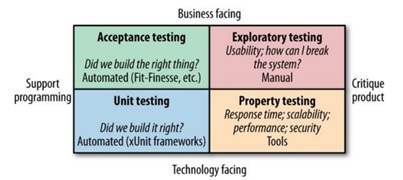
\includegraphics[width=1\textwidth]{test_types.jpg}
    \caption{Rodzaje testów. Źródło: \parencite{newman:2015ap}}
    \label{fig:test-types}
\end{figure}

Dwie kategorie znajdujące się na dole - unit testing oraz property testing - mają 
pomóc deweloperom stworzenie działającego kodu. Tego rodzaju testy mają na celu 
sprawdzenie, czy system nie jest obciążony usterkami związanymi z implementacją. 
Celem testów należących do dwóch kategorii znajdujących się na górze - acceptance 
testing oraz exploratory testing - jest pomoc w zrozumieniu jak dany system działa. 
Do tego rodzaju testów można zaliczyć m. in. szerokie testy obejmujące działanie dużej 
ilości serwisów, sprawdzenie funkcjonalności systemu oraz tzw. „user acceptance 
testing”, czyli testy przeprowadzone przez klienta, który zlecił budowę systemu.

\subsection{Testy jednostkowe}

Tego rodzaju testy sprawdzają poprawność pojedynczej funkcji w kodzie. Nie uruchamia 
się całego serwisu, a jedynie sprawdza jego część. Wszystkie parametry, które 
przyjmuje dana funkcja, są tworzone w trakcie testu. Testy jednostkowe są wykonywane 
w pierwszej fazie testów ze względu na szybkość ich wykonania. Ich celem jest wykrycie 
błędów związanych z daną technologią, nie zaś sprawdzenie, czy działanie systemu jest 
zgodne z oczekiwaniami klienta. Należy zapewnić dużą liczbę testów 
jednostkowych, ponieważ jest to najszybszy sposób zlokalizowania potencjalnych awarii.

Przykładem jest poniższy test:

\begin{lstlisting}
    [Test]
    public void WhenMeasurementsAreTooHigh_ShouldReturnTooHighIndicators()
    {
        // Arrange
        var currentMeasurement = CreateMeasurementSentEvent();
        var policy = TestPoliciesDataService.CreateNewRoomPolicyDto(15, 80, 0.3f, 2, 20, 0.1f);

        // Run
        var result = _policyEvaluator!.Evaluate(currentMeasurement, policy);
        
        // Assert
        Assert.AreEqual(result.TemperatureStatus, EvaluatorResult.TooHigh);
        Assert.AreEqual(result.IlluminanceStatus, EvaluatorResult.TooHigh);
        Assert.AreEqual(result.HumidityStatus, EvaluatorResult.TooHigh);
    }
\end{lstlisting}

Sprawdza on działanie logiki odpowiedzialnej za porównanie aktualnie panujących 
warunków w pomieszczeniu z warunkami oczekiwanymi. Test składa się z trzech części:

\begin{itemize} % lista nienumerowana
    \item Arrange - przygotowanie niezbędnych komponentów potrzebnych do przetestowania 
    fragmentu kodu
    \item Run - faktyczne uruchomienie testowanego kodu
    \item Assert - sprawdzenie otrzymanego wyniku z oczekiwanym rezultatem
\end{itemize}

\subsection{Testy integracyjne}

Testy integracyjne mają na celu sprawdzenie, czy poszczególne mikroserwisy będą 
w stanie się ze sobą skutecznie komunikować. Przykładem jest poniższy test:

\begin{lstlisting}
    [Test]
    public async Task GetExpectedRoomConditions_ShouldBeAvailableUnderDefinedPath()
    {
        var path = $"policies-api/expected-room-conditions/1";
    
        var response = await _client.GetAsync(path);
    
        response.StatusCode.Should().Be(HttpStatusCode.OK);
    }    
\end{lstlisting}

Klient testowy korzysta z oferowanego przez testowany mikroserwis styku poprzez 
wysłanie żądania http. W tym przypadku nie jest testowana logika zawarta w testowanym 
mikroserwisie, a jedynie odpowiedź, którą odsyła. Status odpowiedzi powinien oznaczać 
sukces, sygnalizowany przez kod 200 OK \parencite{fielding:1999ae}.

\subsection{Testy end-2-end}

Testy typu end2-end mają za zadanie przetestować pewne biznesowe 
funkcjonalności, których realizacja może być obsługiwana przez wiele mikroserwisów. 
Dobrą praktyką jest utrzymywanie niewielkiej liczbę tego typu testów, ponieważ 
obejmują one zakres całego systemu i przeprowadzenie każdego z nich zajmuje dużo 
czasu. Ponadto, w przypadku wystąpienia usterki ciężko jest wykryć miejsce, które 
było źródłem błędu.
Przykładem jest poniższy test:

\begin{lstlisting}
def test_measurement_should_trigger_policies_evaluation_result_event():
    new_measurement_test_helper = NewMeasurementTestHelper()

    # check that influxdb is available and bucket exists
    new_measurement_test_helper.check_influxdb_is_available()

    # check that sensors_api is available
    new_measurement_test_helper.check_sensors_api_is_available()

    # send new measurement to rabbitmq
    new_measurement_test_helper.send_new_measurement_to_rabbitmq()

    # check that new measurement has been sent to sensors test queue
    new_measurement_test_helper
    .check_message_sent_to_queue(
        new_measurement_test_helper.rabbitmq_configuration.vhost,
        consts.sensors_test_queue, 
        1)

    # check that MeasurementSentEvent has been sent to test queue  
    new_measurement_test_helper.
    check_message_sent_to_queue(
        new_measurement_test_helper.rabbitmq_configuration.vhost,
        consts.measurement_sent_event_test_queue, 
        1)

    # check that PoliciesEvaluationResultEvent has been sent to test queue
    new_measurement_test_helper.
    check_message_sent_to_queue(
        new_measurement_test_helper.rabbitmq_configuration.vhost,
        consts.policies_evaluation_result_event_test_queue, 
        1)


\end{lstlisting}

W tym teście sprawdza się odpowiedź całego systemu na otrzymanie nowego pomiaru 
z sensora. Jako skutek powinna zostać wygenerowana odpowiednia wiadomość z wynikiem 
przetworzenia pomiaru na kolejce wiadomości.

\subsection{Automatyzacja testów}

Ręczne uruchamianie każdego z testów pojedynczo może szybko stać się żmudnym zajęciem. 
Aby temu zaradzić, w ramach pracy inżynierskiej wykorzystano narzędzie do automatyzacji 
o nazwie Nuke. Za jego pomocą uruchomienie wszystkich testów sprowadza się do wykonania 
jednej komendy. 

Nuke pozwala na tworzenie własnych metod zwanych targetami, które automatyzują 
wykonywanie pewnych czynności. Każdy z targetów wykonują określoną logikę. 
Dodatkowo, można tworzyć kompleksową strukturę, w której każdy z targetów jest zależny 
od tego, czy prawidłowo zostanie wykonany inny target. Istnieje także możliwość 
dodania reguły wyzwalania poszczególnych targetów po wykonaniu innego. 
Przykładowo, metoda uruchamiająca test dla konkretnego projektu wygląda w sposób 
następujący:

\begin{lstlisting}
Target TestProject => _ => _
.DependsOn(CompileTestProject)
.Executes(() =>
{
    var solution = (this as IHaveSolution).Solution;
    var project = solution.AllProjects.Single(x => x.Name == TestProjectNames[ProjectName]);
    DotNet($"test {project} --no-build -c {Configuration}");
});
\end{lstlisting}

Wykonuje ona metodę dotnet test, uruchamianą dla projektu o nazwie ProjectName. 
Target zależy od innej metody o nazwie CompileTestProject.

\begin{lstlisting}
Target CompileTestProject => _ => _
.DependsOn(RestoreTestProject)
.Executes(() =>
{
    var solution = (this as IHaveSolution).Solution;
    var project = solution.AllProjects.Single(x => x.Name == TestProjectNames[ProjectName]);
    DotNetBuild(s => s
        .EnsureNotNull(this as IHaveSolution, (_, o) => s.SetProjectFile(project))
        .SetConfiguration(Configuration)
        .EnableNoRestore());
});
\end{lstlisting}

Metoda wykonuję komenę dotnet build dla projektu o nazwie ProjectName. Jest ona 
zależna od targetu RestoreTestProject.

\begin{lstlisting}
Target RestoreTestProject => _ => _
.DependsOn(Clean)
.Requires(() => ProjectName)
.Executes(() =>
{
    var solution = (this as IHaveSolution).Solution;
    foreach (var proj in solution.AllProjects)
    {
        Logger.Info(proj.Name);
    }
    var project = solution.AllProjects.Single(x => x.Name == TestProjectNames[ProjectName]);
    DotNetRestore(s => s.EnsureNotNull(this as IHaveSolution, (_, o) => s.SetProjectFile(project)));
});
\end{lstlisting}

Metoda wykonuje funkcję dotnet restore na projekcie o nazwie ProjectName. Jednym z 
warunków uruchomienia tego targetu jest konieczność podania nazwy projektu, wyrażona 
przez funkcję .Requires(() => ProjectName). Target jest zależny od innego targetu o 
nazwie Clean.

\begin{lstlisting}
Target Clean => _ => _
.Executes(() =>
{
    SourceDirectory.GlobDirectories("**/bin", "**/obj").ForEach(DeleteDirectory);
    EnsureCleanDirectory(ArtifactsDirectory);
});
\end{lstlisting}

Metoda czyści repozytorium z artefaktów. Nie jest zależna od żadnego innego targetu.
Wszystkie targety można uruchomić przy wykorzystaniu tylko jednej metody:

\begin{lstlisting}
./build.sh TestProject --ProjectName facilities --verbosity verbose
\end{lstlisting}

\section{Pomiary}

W ramach tej pracy inżynierskiej przygotowano zestaw pomiarowy, który 
w regularnych odstępach czasu bada aktualną wartość temperatury oraz
natężenia światła. Zestaw został złożony z następujących elementów:

\begin{itemize} % lista nienumerowana
    \item Moduł WEMOS D1 Uno R3 ESP8266 WIFI
    \item Fotorezystor LDR GL5528
    \item Czujnik temperatury i wilgotności DHT11
    \item Rezystory 1 kOhm
\end{itemize}

Moduł WEMOS jest mikrokontrolerem oparty o kontroler ATmega328P. Posiada
11 portów wejścia-wyjścia pozwlających na dołączenie zewnętrznych 
urządzeń. Płytka została fabrycznie wyposażona w moduł wifi ESP8266. Za
jego pomocą mogą zostać wysłane pomiary.

Fotorezystor służy do pomiaru natężenia światła. Został wykonany 
z półprzewodników, które w temperaturze działania nie mają elektronów 
w paśmie przewodnictwa. Padające na półprzewodnik fotony o energii 
większej od przerwy energetycznej przemieszczają elektrony z pasma 
walencyjnego do pasma przewodnictwa, w wyniku którego powstają pary 
dziura-elektron. Zjawisko nazywane jest efektem fotoelektrycznym 
wewnętrznym.

Czujnik temperatury i wilgotności DHT11 bada aktualne wartości tych
dwóch parametrów. Mierzony zakres temperatury to -20\degree  - +60\degree C.
Jego rozdzielczość wynosi 0.1\degree C, a dokładność 2\degree C.

\subsection{Oprogramowanie mikrokontrolera}

Do rozwoju oprogramowania do mikrokontrolera WEMOSC wykorzystano narzędzie 
Arduino IDE, będące rozbudowanym edytorem pozwalającym na kompilację,
przesyłanie plików wykonywalnych na płytkę przy pomocy kabla USB oraz
debugowanie i podgląd logów produkowanych przez mikrokontroler w czasie 
rzeczywistym. Do utworzeniu kodu został wykorzystany język C.

Zadaniem mikrokontrolera było:

\begin{itemize} % lista nienumerowana
    \item Zebranie aktualnych pomiarów temperatury i natężenia światła
    \item przygotowanie wiadomości z uzyskanymi pomiarami
    \item wysłanie wiadomości przy pomocy protokołu MQTT przez moduł WIFI na 
    kolejkę brokera wiadomości RabbitMQ
\end{itemize}

Poniżej został przedstawiony przygotowany kod.

\begin{lstlisting}
    #include "rabbitmq_handler.h"

    #define WIFI_SSID "Tech_D0054234"
    #define WIFI_PASS "PASSWORD"
     
    void setup() {
      Serial.begin(115200);
      dht.begin();
      Serial.println();
     
      WiFi.mode(WIFI_STA);
      WiFi.begin(WIFI_SSID, WIFI_PASS);
     
      while (WiFi.status() != WL_CONNECTED)
      {
        delay(100);
      }
      
      client.setServer(RABBITMQ_BROKER, RABBITMQ_PORT);
      client.setCallback(callback);
    }
     
    void loop() {
      if ( !client.connected() ) {
        reconnect();
      }
      
      float temperature = readTemperature(&dht);
      int illuminance = analogRead(ILLUMINANCEPIN);
      publish_measurements(temperature, illuminance, false);
      
      delay(60000);
    
      client.loop();
    }
\end{lstlisting}

Każdy z programów wgrywanych na płytkę powinien zawierać dwie główne funkcje:

\begin{itemize}
    \item void setup() - wewnątrz metody definiowane są obiekty oraz zmienne 
    potrzebne przez cały czas działania mikrokontrolera
    \item void loop() - metoda wywoływana jako druga w kolejności po setup(),
    jest powtarzana przez resztę cyklu działania mikrokontrolera 
\end{itemize}

Na początku definiowana jest szyna, za pomocą której przesyłane są dane do 
modułu WIFI. Moduł wspiera prędkość transmisji na poziomie 115200 bitów na 
sekundę (ang. baud rate). Następnie tworzony jest klient, którego zadaniem
jest wysyłanie pomiarów na kolejkę brokera wiadomości. 

Wewnątrz metody loop() co 60 sekund zbierane są pomiary, po czym publikowane
na kolejkę. Pomiary wykonywane są przy użyciu poniższego kodu.

\begin{lstlisting}
    #include "DHT.h"

    #define DHTPIN 4
    #define DHTTYPE DHT11
    
    int ILLUMINANCEPIN = A0;
    
    DHT dht(DHTPIN, DHTTYPE);
    
    float readTemperature(DHT *dht){
      float t = dht->readTemperature();
     
      if (isnan(t))
      {
        Serial.println("Error while reading current temperature value");
      }
      
      return t;
    }
\end{lstlisting}

Główną rolę pełni obiekt dht, za pomocą którego można komunikować się
z czujnikiem. Zdefiniowany jest typ czujnika przy użyciu makra DHTTYPE.
Numer pinu, do którego został wpięty kabel łączący płytkę z czujnikiem,
został oznaczony pzy użyciu makra DHTPIN. Pomiar temperatury odbywa się
przez wywołanie funkcji readTemperature(). 

Pomiar z fotorezystora można odczytać przy użyciu komendy:  

\begin{lstlisting}
    analogRead(ILLUMINANCEPIN)
\end{lstlisting}

gdzie ILLUMINANCEPIN oznacza numer pinu, do 
którego wpięty jest kabel łączący płytkę z fotorezystorem.

Poniższy kod zawiera szczegóły implementacyjne dotyczące 
wysyłania wiadomości na kolejkę.



Warto wyjaśnić wartości zmiennych związanych z brokerem wiadomości:
\begin{lstlisting}
    const char* RABBITMQ_BROKER = "192.168.0.12";
    int        RABBITMQ_PORT     = 1883;
    const char* RABBITMQ_TOPIC  = "room_measurements";
    const char* RABBITMQ_SUBSCRIPTION  = "request_measurement";
    const char* RABBITMQ_USER = "guest";
    const char* RABBITMQ_PASSWORD = "guest";
    const char* RABBITMQ_SENSOR_ID = "968376";
\end{lstlisting}

\begin{itemize}
    \item RABBITMQ\_BROKER: adres IP serwera, na którym uruchomiony jest broker wiadomości
    \item RABBITMQ\_PORT: numer portu serwera, na którym nasłuchuje broker
    \item RABBITMQ\_TOPIC: temat, na który wysyłane są wiadomości z mikrokontrolera
    na kolejkę
    \item RABBITMQ\_SUBSCRIPTION: temat, na który nasłuchuje mikrokontroler
    \item RABBITMQ\_USER: nazwa użytkownika, za pomocą którego płytka jest uwierzytelniana
    \item RABBITMQ\_PASSWORD: hasło dla wykorzystywanego użytkownika
\end{itemize}

Wiadomość do brokera jest wysyłana w metodzie send\_measurements:

\begin{lstlisting}
    void send_measurements(float temperature, int illuminance){
      char temperatureChar[64];
      int ret = snprintf(temperatureChar, sizeof temperatureChar, "%f", temperature);
      if (ret < 0) {
          return;
      }
      if (ret >= sizeof temperatureChar) {
           return;
      }
      char illuminanceChar[64];
      ret = snprintf(illuminanceChar, sizeof illuminanceChar, "%d", illuminance);
      if (ret < 0) {
          return;
      }
      if (ret >= sizeof illuminanceChar) {
           return;
      }
    
      char* measurement = (char*)malloc(256+1+3); //4*64 + 3 semicolons + EOF
      strcpy(measurement, temperatureChar);
      strcat(measurement, ";");
      strcat(measurement, illuminanceChar);
      strcat(measurement, ";");
      strcat(measurement, RABBITMQ_SENSOR_ID);
    
      time_t t = time(NULL);
      struct tm tm = *localtime(&t);
    
      client.publish(RABBITMQ_TOPIC, measurement);
    
      free(measurement);
    }
\end{lstlisting}

Mikrokontroler nasłuchuje na wiadomości o temacie RABBITMQ\_SUBSCRIPTION:

\begin{lstlisting}
    void callback(char* topic, byte* payload, unsigned int length) {
      char* sensorId = (char*)payload;
    
      String messageTemp;
      
      for (int i = 0; i < length; i++) {
        Serial.print((char)payload[i]);
        messageTemp += (char)payload[i];
      }
    
      if(strcmp(topic, RABBITMQ_SUBSCRIPTION) == 0 && strcmp(sensorId, RABBITMQ_SENSOR_ID)){
        float temperature = readTemperature(&dht);
        int illuminance = analogRead(ILLUMINANCEPIN);
        publish_measurements(temperature, humidity, illuminance, true);
      }
    }
\end{lstlisting}

\section{Automatyzacja}

Pełna automatyzacja regularnie wykonywanych zadań, pozwalająca znacznie przyspieszyć 
wdrażanie całości systemu, była jednym z najważniejszych zagadnień poruszonych w 
trakcie tworzenia pracy. Prawidłowe podejście do wdrażania aplikacji znacząco wpływa 
na szybkość, z jaką zmiany wprowadzone lokalnie mogą zostać wykorzystane w 
produkcyjnej wersji systemu. 

\subsection{Docker}

Docker jest otwartą platformą do rozwoju oraz wdrażania aplikacji. Pozwala oddzielić aplikacje od
dostępnej na danym serwerze infrastruktury, co pozwala przyspieszyć proces dostarczania najnowszych
wersji systemów. 

Platforma pozwala zapewnia możliwość spakowania i uruchomienia aplikacji w odizolowanym środowisku
zwanym kontenerem. Izolacja powoduje, że możliwe jest bezpieczne uruchomienie wielu kontenerów na tym
samym hoście. Platforma pozwala zarządzać infrastrukturą potrzebną do uruchomienia kontenera, dzięki
czemu eliminowany jest problem instalacji wszystkich wymaganych zależności na każdym serwerze z osobna.

Docker wykorzystuje architekturę typu klient-serwer. Klient komunikuje się z tzw. docker daemon, którego
zadaniem jest budowanie, uruchamianie oraz dystrybuowanie kontenerów. 

W celu utworzenia kontenerów należy w pierwszej kolejności utworzyć ich obraz, który jest szablonem
zawierającym instrukcje dotyczące budowy. Szablony są przechowywane w plikach o nazwie Dockerfile.
Każda instrukcja tworzy jedną warstwę obrazu. Mechanizm ten jest szczególnie przydatny, gdy szablony są
regularnie rozwijane o nowe instrukcje. Wtedy, przy ponownym budowaniu obrazu, tylko warstwy, które
uległy zmianie są odświeżane. Pozwala to znacznie przyspieszyć proces budowania obrazów.

Kontener jest instancją obrazu, którą można uruchomić. Działa on tak długo, dopóki nie zostanie
zakończony proces główny.

Przykładowy szablon, który przedstawia obraz Addresses Data Service, został przedstawiony poniżej:

\begin{lstlisting}
FROM mcr.microsoft.com/dotnet/aspnet:5.0 AS base
WORKDIR /app
EXPOSE 80
EXPOSE 443

FROM mcr.microsoft.com/dotnet/sdk:5.0 AS build
WORKDIR /app
COPY ["./DagAir_Addresses/DagAir.Addresses/", "./DagAir_Addresses/DagAir.Addresses/"]
COPY ["./DagAir_Addresses/DagAir.Addresses.Data/", "./DagAir_Addresses/DagAir.Addresses.Data/"]
COPY ["./DagAir_Addresses/DagAir.Addresses.Contracts/", "./DagAir_Addresses/DagAir.Addresses.Contracts/"]
COPY ["./DagAir_Components/DagAir.Components.ApiModels/", "./DagAir_Components/DagAir.Components.ApiModels/"]
COPY ["./DagAir_Components/DagAir.Components.Healthchecks/", "./DagAir_Components/DagAir.Components.Healthchecks/"]
COPY ["./DagAir_Components/DagAir.Components.Logging/", "./DagAir_Components/DagAir.Components.Logging/"]

RUN dotnet restore ./DagAir_Addresses/DagAir.Addresses/DagAir.Addresses.csproj
RUN dotnet build ./DagAir_Addresses/DagAir.Addresses/DagAir.Addresses.csproj --no-restore
RUN dotnet publish ./DagAir_Addresses/DagAir.Addresses/DagAir.Addresses.csproj -c Release -o /app/publish

FROM base AS final
WORKDIR /app
COPY --from=build /app/publish .

ENTRYPOINT ["dotnet", "DagAir.Addresses.dll"]
\end{lstlisting}

Pierwszym etapem jest utworzenie obrazu pośredniego o nazwie base. Oparty on jest na obrazie 
aspnet:5.0 dostępnym publicznie na platformie 
\href{https://hub.docker.com/_/microsoft-dotnet-aspnet}{dockerhub}. Na tym etapie deklarowane są
numery portów, na których aplikacja powinna nasłuchiwać na przychodzące żądania.

Drugim etapem jest utworzenie obrazu pośredniego, opartego o obraz sdk:5.0, również dostępnym publicznie
na platformie \href{https://hub.docker.com/_/microsoft-dotnet-sdk}{dockerhub}. Na tym etapie kopiowane
są wszystkie zależności, których wymaga aplikacja, by mogła zostać prawidłowo uruchomiona.
Za pomocą komend oferowanych przez dotnet CLI publikowana jest gotowa do wdrożenia wersja aplikacji.

W ostatnim etapie kopiowana jest wersja aplikacji przygotowana w ramach etapu drugiego, po czym
następuje uruchomienie procesu za pomocą komendy:

\begin{lstlisting}
    dotnet DagAir.Addresses.dll
\end{lstlisting}

Podział na poszczególne etapy wynika z różnych rozmiarów wykorzystywanych obrazów. Możliwe byłoby
utworzenie obrazu aplikacji na podstawie obrazu sdk:5.0. Jednak jego rozmiar to ok. 630 MB, podczas
gdy rozmiar obrazu aspnet:5.0 to ok. 205 MB. Dzięki temu prostemu zabiegowi można oszczędzić 
znaczne zasoby obliczeniowe. 

Dzięki szablonom można tworzyć obrazy poszczególnych serwisów. Jednak uruchamianie każdego z nich
pojedynczo byłoby kosztownym czasowo zajęciem. Rozwiązaniem tego problemu jest wykorzystanie narzędzia
docker-compose, które umożliwia uruchamianie wielu kontenerów za pomocą jednej komendy. W tym celu
należy przygotować szablon zawierający instrukcje uruchomienia każdego z utworzonych na wcześniejszym
etapie obrazów. Szablon jest przechowywany w pliku o nazwie docker-compose.yml.

Przykładowy szablon został przedstawiony poniżej:

\begin{lstlisting}
    version: "3.9"

    services:
      addresses_api:
        build:
          target: final
          context: ./src
          dockerfile: ./DagAir_Addresses/Dockerfile
        environment:
          - ASPNETCORE_ENVIRONMENT=Docker
          - ConnectionKeys__DagAir.Addresses=
                ${ADDRESSES_CONNECTIONKEYS}
        ports:
          - "8094:80"
        networks:
          - dagair_network
        restart: always

    networks:
    dagair_network:
\end{lstlisting}

W szablonie został przedstawiony proces uruchomienia Addresses Data Service. Zdefiniowano:

\begin{itemize}
    \item Szablon obrazu, z którego należy skorzystać
    \item Zmienne środowiskowe potrzebne do uruchumienia aplikacji w środowisku dockerowym
    \item Port, na którym ma nasłuchiwać aplikacja. Występuje tutaj mapowanie między portem 
    serwera, na którym będzie uruchomiony kontener, a portem w kontenerze. Dzięki mapowaniu
    aplikacja będzie dostępna na serwerze pod adresem:

    \begin{lstlisting}
        http://localhost:8094/
    \end{lstlisting}
    \item Wirtualna sieć, do którego ma zostać dołączony kontener w środowisku dockerowym
    \item Polityka ponownego uruchamiania. Flaga always oznacza, że w przypadku zatrzymania pracy
    instancji kontenera, zostanie ona usunięta, a na jej miejsce zostanie uruchomiona nowa
\end{itemize}


\subsection{Ciągła integracja}

Podstawowym wymaganiem, które należy spełnić przy tworzeniu rozbudowanych systemów 
informatycznych, jest przechowywanie rozwijanego oprogramowania przy pomocy wybranego 
narzędzia kontroli wersji, takiego jak Git. Dane są zapisywane w folderze zwanym 
również repozytorium. Zadaniem takiego narzędzia jest śledzenie wprowadzonych zmian 
oprogramowania i zapisywanie ich w historii repozytorium. Zapewnia to wiele 
korzyści, z których najważniejsze to:

\begin{itemize} % lista nienumerowana
    \item Podgląd zmian wprowadzonych przez każdego dewelopera
    \item Możliwość powrotu do poprzedniej wersji w przypadku, gdy wprowadzone zmiany 
    były przyczyną błędów w działaniu systemu
\end{itemize}

Głównym celem ciągłej integracji (ang. continuous integration) jest regularne włączanie 
bieżących zmian w kodzie do głównego repozytorium i każdorazowa weryfikacja 
wprowadzonych zmian poprzez utworzenie nowego zbioru plików wykonywalnych 
i przeprowadzenie na nich testów jednostkowych. Zaletą tego podejścia jest fakt, że 
po wysłaniu przez programistę zmian do repozytorium głównego, reszta czynności 
wykonywana jest automatycznie przez serwer ciągłej integracji, bez ingerencji 
człowieka. Dodatkowo programista otrzymuje szybką odpowiedź zwrotną w razie 
wystąpienia błędów.
Aby wykorzystać potencjał ciągłej integracji, należy zwrócić uwagę na następujące 
punkty: 

\begin{itemize} % lista nienumerowana
    \item Częste i regularne wysyłanie kodu do głównego repozytorium w celu weryfikacji 
    integracji nowych zmian z resztą kodu, przynajmniej raz dziennie 
    \item Zapewnienie testów jednostkowych sprawdzających poprawność zachowania systemu. 
    Może się zdarzyć, że wprowadzone zmiany będą zgodne pod względem 
    syntaktycznym, jednak nie oznacza to, że serwis będzie prawidłowo spełniał swoje 
    funkcje 
    \item Nadanie wysokiego priorytetu naprawieniu kodu, który nie integruje się z 
    dotychczasowym kodem w repozytorium. Odkładanie poprawy na później może spowodować 
    spiętrzenie się kolejnych błędów, co w konsekwencji bardziej spowolni wdrażanie 
    nowych funkcji
\end{itemize}

W trakcie tworzenia pracy wykorzystano platformę do ciągłej integracji i wdrażania 
o nazwie Github Actions. Pozwala ona na automatyzację tworzenia nowych wersji 
oprogramowania, testowania oraz wdrażania. Kolejne powtórzenia przepływów pracy 
(ang. workflow) są wykonywane na maszynach wirtualnych oferowanych przez 
GitHub, zwanych pracownikami (ang. worker). W zależności od potrzeby na maszynach 
zainstalowany jest odpowiedni system operacyjny spośród sytrybucji 
linux-owych, Windowsa oraz macOS.

GitHub Action jest przepływem pracy, który może zostać wywołany zawsze wtedy, gdy 
zostanie zarejestrowane nowe zdarzenie dotyczące wykorzystywanego repozytorium. 
Przykładem zdarzenia jest wprowadzenie nowych zmian do repozytorium lub utworzenie 
żądania typu pull request. GitHub Action składa się z jednej lub większej liczby 
zadań (ang. job), które mogą zostać wykonane jedno po drugim lub równolegle. Z kolei 
każde zadanie składa się z jednego lub większej liczby kroków (ang. step), z których 
każde może wykonać własnoręcznie utworzony skrypt lub akcję (ang. action), która jest 
rozszerzeniem umożliwiającym na uproszczenie całego przepływu pracy.

Przykładowy przepływ pracy utworzony na potrzeby pracy wykonuje następujące zadania:

\begin{itemize} % lista nienumerowana
    \item Wybiera odpowiednią gałąź z repozytorium, na której zostały wprowadzone 
    nowe zmiany
    \item Instaluje wymagane oprogramowanie niezbędne do wykonania wszystkich 
    pozostałych zadań, takie jak wersja .NET 5.0
    \item Uruchamia testy jednostkowe i integracyjne
    \item Tworzy nową wersję obrazu przestestowanego mikroserwisu
    \item Wypycha obraz do rejestru kontenerów
\end{itemize}

Warto szczegółowo prześledzić poszczególne kroki danego przepływu.

\begin{lstlisting}
jobs:
  docker-build-and-push:
    runs-on: ubuntu-latest
    steps:
    - name: Checkout
      uses: actions/checkout@v2
      with:
        fetch-depth: 0
\end{lstlisting}

Powyższy wyciąg deklaruje nowe zadanie oraz pierwszy z kroków, który wybierze 
odpowiędnią gałąź z repozytorium. Parametr runs-on wskazuje jaki rodzaj systemu 
operacyjnego powinien zostać wykorzystany.

\begin{lstlisting}
on:
  workflow_dispatch: # allows to trigger workflow on demand
  push:
    branches: 
      - main
      - develop
    paths:
      - src/DagAir_Facilities/**
\end{lstlisting}

GitHub Actions oferuje rozbudowany system do określania warunków, które muszą być 
spełnione, aby uruchomić przepływ pracy. Powyższy wyciąg przedstawia fragment, który 
określa, że przepływ ma być uruchomiony gdy:

\begin{itemize} % lista nienumerowana
    \item Użytkownik manualnie uruchomi przepływ za pomocą interfejsu graficznego
    \item Zostaną wprowadzone nowe zmiany na gałęzi main lub develop oraz zmiany będą 
    się znajdować w katalogu src/DagAir\_Facilities/
\end{itemize}

\begin{lstlisting}
- name: Build & Test
    shell: bash
    run: ./build.sh TestProject --ProjectName facilities --verbosity verbose
\end{lstlisting}

Powyższy krok wykonuje skrypt uruchamiający testy jednostkowe oraz integracyjne.

\begin{lstlisting}
- name: Set image names & main tags
run: |
  appImageName="${{ env.CONTAINER_REGISTRY }}/${{ env.SERVICE_NAME }}"
  migrationsApplierImageName="${{ env.CONTAINER_REGISTRY }}/${{ env.MIGRATIONS_APPLIER_NAME }}"
  echo "APP_IMAGE_NAME=$appImageName" >> $GITHUB_ENV
  echo "MIGRATIONS_APPLIER_IMAGE_NAME=$migrationsApplierImageName" >> $GITHUB_ENV

  version="${{ steps.gitversion.outputs.nugetVersionV2 }}-${{ steps.gitversion.outputs.shortSha }}"

  if [ ${{ steps.gitversion.outputs.commitsSinceVersionSource }} -gt 0 ]; then
  version="${{ steps.gitversion.outputs.escapedBranchName }}-$version"
  fi

  echo "APP_IMAGE_TAG=${appImageName}:$version" >> $GITHUB_ENV
  echo "MIGRATIONS_APPLIER_IMAGE_TAG=
  ${migrationsApplierImageName}:$version" \
  >> $GITHUB_ENV
\end{lstlisting}

Powyższy krok generuje nazwę oraz tag nowego obrazu testowanego mikroserwisu. Na nazwę 
obrazu składa się nazwa repozytorium obrazów oraz nazwa mikroserwisu. Numer wersji 
obrazu za każdym razem powinien być unikalny, ponadto powinien wskazywać, która z 
wersji obrazu jest najnowsza. Wobec tego na wersję składa się nazwa gałęzi 
repozytorium, nazwa utworzonej paczki Nuget-owej oraz krótki unikalny numer przypisany 
do commit'a, który spowodował uruchomienie przepływu.

\begin{lstlisting}
- name: Docker login
  uses: docker/login-action@v1
  with:
    registry: ${{ env.CONTAINER_REGISTRY }}
    username: ${{ secrets.AZURE_CR_USERNAME }}
    password: ${{ secrets.AZURE_CR_PASSWORD }}

- name: Docker push images
  run: |
    docker push ${{ env.APP_IMAGE_NAME }} --all-tags
    docker push ${{ env.MIGRATIONS_APPLIER_IMAGE_NAME }} --all-tags
\end{lstlisting}

Na samym końcu gotowy obraz zostaje wypchnięty do repozytorium obrazów. W tym celu 
używana jest komenda docker push. Aby zakończyła się pomyślnie, trzeba było 
w poprzednim kroku zalogować się, wykorzystując nazwę repozytorium obrazów oraz 
danych uwierzytelniający, przechowywanych w bezpieczny sposób za pomocą Github 
Secrets.

\subsection{Ciągłe dostarczanie}

W trkacie prac nad systemem wykorzystano metodykę ciągłego dostarczania, które polega na tym, że kod 
przechodzi przez kolejne fazy testowania, gdzie za każdym razem jest weryfikowana jego poprawność pod 
względem prawidłowego funkcjonowania. 

Na początku przeprowadzane są szybkie testy jednostkowe sprawdzające punktowo poprawność 
poszczególnych funkcji. Jeśli zostaną wykonane pomyślnie, przechodzi się do następnej fazy 
testowania uwzględniające wolniejsze testy, które sprawdzają zachowanie wielu serwisów między 
sobą. Po upewnieniu się, że ta faza została wykonana pomyślnie, system jest weryfikowany przez 
klienta, który zlecał jego wykonanie (tzw. „user acceptance testing”). Jeśli funkcjonalność zgadza się z 
oczekiwaniami klienta, całość jest jeszcze testowana pod kątem wydajności, po czym zostaje 
wdrożona na etap produkcyjny.
Zgodnie z założeniami metodyki, programiści powinni otrzymywać
wiadomości zwrotne dotyczące statusu kolejnych wersji 
oprogramowania w kolejnych fazach testowania. Wprowadzenie takiego potoku potrafi znacznie
poprawić ocenę jakości kodu, ponadto skrócić czas między wdrożeniem kolejnych wersji systemu.

\subsection{Kubernetes}

Kubernetes jest platformą do orkiestracji kontenerów automatyzującą procesy manualne 
związane z wdrażaniem, zarządzaniem oraz skalowaniem skonteneryzowanych aplikacji. 
Jest to oprogramowanie typu open-source, początkowo rozwijane przez firmę Google.

W przeszłości, organizacje uruchamiały aplikacje na fizycznych serwerach. W momencie 
gdy wiele aplikacji działało w ramach jednego serwera, dochodziło do 
sytuacji, w których jedna z aplikacji zajmowała większość zasobów, przez co inne 
aplikacje nie działały optymalnie. Jednym z rozwiązań było uruchomienie każdej 
z aplikacji na innym fizycznym serwerze. Jednak w takim wypadku konsekwencjami były 
wysokie koszty utrzymania infrastruktury. Innym możliwym rozwiązaniem było wprowadzenie 
wirtualizacji, które przyczyniło się do bardziej zrównoważonego zarządzania zasobami. 
Efektem ubocznym było jednak wprowadzanie dużego nakładu zasobów potrzebnych na 
uruchomienie samej maszyny wirtualnej, ponieważ każda z maszyn instalowała na początku 
własny system operacyjny.

Najlepszym obecnie rozwiązaniem jest wykorzystanie kontenerów. Zawierają zestaw 
podobnych cech do maszyn wirtualnych z tą różnicą, że nie wymagają osobnego systemu 
operacyjnego. Każdy z kontenerów może współdzielić jeden system operacyjny z 
innymi, co znacznie obniża wymagania dotyczące zasobów. Podobnie do maszyn 
wirtualnych posiadają własny system plików, zasoby obliczeniowe, pamięć. Jednak nie 
zależą od infrastruktury, na której są uruchamiane, co czyni je przenośnymi wśród 
różnych dystrybucji danego systemu.

Kontenery stały się popularne ze względu na szereg zalet:

\begin{itemize} % lista nienumerowana
    \item Utworzenie obrazów następuje szybciej w porównaniu do maszyn wirtualnych
    \item Utworzenie obrazów na etapie budowania nowej wersji systemu zamiast na etapie wdrażania
    \item Niezależnie od środowiska działa w dokładnie ten sam sposób
    \item Mogą być uruchomione praktycznie na każdym systemie i dystrybucji
    \item Wysoka efektywność wykorzystania zasobów
\end{itemize}

Rysunek \ref{fig:deployment-types}. przedstawia różnice między uruchomieniem aplikacji w sposób 
tradycyjny, przy użyciu maszyn wirtualnych oraz kontenerów.

\begin{figure}[h]
    \centering
    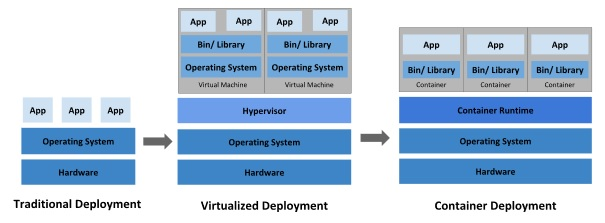
\includegraphics[width=1\textwidth]{deployment_types.jpg}
    \caption{Porównanie różnych metod uruchamiania aplikacji. Źródło: \href{https://kubernetes.io/docs/concepts/overview/what-is-kubernetes/}{What is Kubernetes?}}
    \label{fig:deployment-types}
\end{figure}

Zalety Kubernetesa to przede wszystkim:

\begin{itemize} % lista nienumerowana
    \item Orkiestracja kontenerów między różnymi serwerami
    \item Efektywniejsze wykorzystanie zasobów
    \item Łatwe skalowanie skonteneryzowanych aplikacji 
    \item Zarządzanie serwisami w sposób deklaratywny
    \item Kontrola stanu aplikacji, automatyczne restartowanie kontenerów, 
    autoskalowanie
\end{itemize}

Zbiór hostów wykorzystywanych do uruchomienia na nich systemu zwany jest klastrem. Na 
każdym z hostów, zwanych węzłami, można uruchomić instancje gotowych obrazów. Każdy 
z klastrów posiada przynajmniej jeden węzeł.

Cyklem życiowym każdego kontenera zarządza płaszczyzna sterowania (ang. control 
plane), która wystawia API oraz interfejsy umożliwiające ich wdrażanie i zarządzanie. 
Komponenty płaszczyzny mogą być uruchomione na każdej maszynie w klastrze, chociaż 
zazwyczaj określa się jedną maszynę gospodarza (ang. master), na której znajdują się 
wszystkie komponenty.

\subsubsection{Komponenty płaszczyzny sterowania}

W tej części zostały opisane komponenty składające się na całość płaszczyzny 
sterowania.

kube-apiserver - interfejs pozwalający na interakcję z płaszczyzną sterowania. 
Weryfikuje i konfiguruje dane dla obiektów takich jak serwisy czy kontrolery 
replikacji. 

Etcd - to spójny i wysoce dostępny magazyn par klucz-wartość używany przez Kubernetesa 
jako miejsce do przechowywania wszystkich danych ważnych z punktu widzenia klastra. 

Kube-scheduler - regularnie sprawdza czy został utworzony nowy zestaw 
kontenerów, któremu nie został jeszcze przypisany węzeł. W takim przypadku wybiera 
on maszynę, na której kontenery mają być uruchomione. Przy wyborze pod uwagę brane są 
takie czynniki jak wymagane zasoby, ograniczenia sprzętowe lub programowe.

Kube-controller-manager - komponent odpowiedzialny za uruchamianie kontrolerów, które 
monitorują oraz zmieniają stan klastra korzystając z API serwera. Istnieje kilka 
rodzajów kontrolerów:

\begin{itemize} % lista nienumerowana
    \item Kontroler węzłów (ang. node controller) - odpowiedzialny za wykrycie oraz 
    odpowiednią reakcję w przypadku, gdy jeden z węzłów ulega awarii lub staje się 
    niedostępny
    \item Kontroler prac (ang. job controller) - nasłuchuje na pojawienie się obiektów 
    pracy (job objects) reprezentujących zadania, a następnie tworzy zbiór (pod) który 
    te zadania wykona
    \item Kontroler punktów końcowych - zarządza obiektami punktów końcowych (serwisy 
    oraz zbiory (ang. pods))
    \item Kontroler kont oraz tokenów - tworzy domyślne konta oraz tokeny dostępu do 
    API dla nowych przestrzeni nazw
\end{itemize}

Cloud-controller-manager - element, który wbudowuje logikę związaną z konkretną 
chmurą, w której tworzone są klastry. Pozwala połączyć dany klaster z API dostawcy 
chmury oraz oddziela komponenty, które oddziałują z chmurą od komponentów, które 
oddziałują tylko z klastrem. Jest to komponent, który występuje tylko w przypadku 
stawiania kontenerów w chmurze. Jeśli Kubernetes działa np. w prywatnym środowisku 
na jednym komputerze, wtedy klaster nie posiada tego elementu. 
Cloud-controller-manager może zapewniać poniższe zależności:

\begin{itemize} % lista nienumerowana
    \item Kontroler węzłów (node controller) - sprawdza czy węzeł został usunięty 
    z chmury po tym jak przestał odpowiadać na żądania
    \item Kontroler routingu (route controller) - zapewnia możliwość ustalenia ścieżek 
    między poszczególnymi elementami infrastruktury chmurowej
    \item Kontroler serwisów (service controller) - zapewnia możliwość 
    tworzenia, edytowania oraz usuwania load balancer-ów
\end{itemize}


\subsubsection{Komponenty węzła}

Poniżej opisano komponenty, które działają na każdym węźle w Kubernetesie.

Kubelet - agent, którego rolą jest upewnienie się, że kontenery są uruchomione 
w zbiorze (pods). Przyjmuje zestaw specyfikacji zbiorów i zapewnia, że wszystkie 
kontenery podane w specyfikacji działają i są sprawne. Kubelet nie zarządza 
kontenerami, które nie zostały utworzone przez Kubernetesa.

Kube-proxy - proxy sieciowe, które implementuje część serwisu pozwalającego wystawić 
aplikację do świata zewnętrznego. Jego zadaniem jest utrzymanie reguł sieciowych 
w zarządzanych węzłach. Te reguły pozwalają na komunikację między różnymi zbiorami 
wewnątrz lub na zewnątrz klastra.

Container runtime - oprogramowanie odpowiedzialne za uruchamianie kontenerów. 
Kubernetes wspiera wiele możliwych runtime'ów, m. in. Docker, containerd, CRI-O.

Pod - grupa złożona z jednego lub większej liczby kontenerów, wdrożona na tym samym 
węźle. Wszystkie kontenery z grupy współdzielą adres IP oraz przydzielone zasoby.

Replication controller - narzędzie do kontroli liczby kopii danego poda, które powinny 
być w danej chwili uruchomione

Płaszczyzna sterowania przyjmuje komendy od administratora klastra, po czym przekazuje 
je do podległych serwerów. Komendy przyjmowane są za pomocą interfejsu 
konsolowego, zwanego kubectl. Dobrą praktyką jest utworzenie plików deklarujących 
pożądany stan, w jakim powinien znajdować się klaster. Przykładowa deklaracja znajduje 
się poniżej.

\begin{lstlisting}
apiVersion: apps/v1
kind: Deployment
metadata:
  name: web-admin-app
  labels:
    app: web-admin-app
    tier: backend
spec:
  replicas: 2
  selector:
    matchLabels:
      app: admin-application-service
  template:
    metadata:
      labels:
        app: admin-application-service
        tier: backend
    spec:
      containers:
      - name: admin-application-service
        image: admin-application-service:develop-latest
        env:
        - name: ASPNETCORE_ENVIRONMENT
          value: "Kubernetes"
        imagePullPolicy: Always
        ports:
        - containerPort: 80

\end{lstlisting}

Jest to deklaracja typu Deployment, która powinna zawierać następujące parametry:

\begin{itemize} % lista nienumerowana
    \item Wersja wykorzystywanego API
    \item Typ deklaracji
    \item Nazwa deklaracji
    \item Specyfikacja przedstawiająca pożądany stan, w jakim powinien znajdować się 
    klaster. W tym przypadku deklaruje się, że w klastrze powinny działać dwie 
    instancje obrazu mikrousługi aplikacyjnej dla administratorów, które powinny 
    nasłuchiwać na żądania na porcie 80
\end{itemize}

Deklarację można zaaplikować korzystając z komendy:

\begin{lstlisting}
kubectl apply -f deployment.yml
\end{lstlisting}

Płaszczyzna sterowania jest odpowiedzialna za to, by stan klastra odpowiadał 
deklaracji. W konsekwencji zostaną utworzone dwa osobne pody, z których każdy otrzyma 
unikalny prywatny adres IP wewnątrz klastra. Od tej pory do każdej instancji można 
się odwołać, wykorzystując jej adres IP oraz numer portu.

Należy wziąć pod uwagę, że pody nie są trwałymi zasobami. Mogą być tworzone i usuwane 
w sposób dynamiczny. Za każdym razem pod otrzymuje nowy adres IP, który może się 
różnić od poprzednich. Prowadzi to do problemów przy komunikacji między 
mikroserwisami, ponieważ nie wiedzą, że wymagany serwis nie jest już osiągalny pod 
dotychczasowym adresem.

Rozwiązaniem tego zagadnienia jest wprowadzenie tzw. serwisu. Jest to abstrakcyjny 
obiekt, który definiuje zbiór pod-ów oraz reguły umożliwiające do nich dostęp. 
Serwisowi nadawany jest unikalny adres IP, pod który mogą odwoływać się mikroserwisy. 
W dalszym ciągu pod-y będą dynamicznie tworzone i usuwane, jednak w tym wypadku będą 
one ciągle dostępne pod adresem IP serwisu.

Przykładem jest poniższa deklaracja:

\begin{lstlisting}
apiVersion: v1
kind: Service
metadata:
  name: admin-application-service
  labels:
    app: admin-application-service
    tier: backend
spec:
  selector:
    app: admin-application-service
  type: LoadBalancer
  ports:
  - port: 8085
    targetPort: 80
    protocol: TCP
    name: http 
\end{lstlisting}

Jest to deklaracja typu Service, która powinna zawierać następujące parametry:

\begin{itemize} % lista nienumerowana
    \item Wersja wykorzystywanego API
    \item Typ deklaracji
    \item Nazwa deklaracji
    \item Selektor. Od niego zależy, które pod-y zostaną dołączone do zbioru
    \item Typ publikacji
    \item Porty
\end{itemize}

Wyróżnia się trzy główne typy publikacji serwisu:

\begin{itemize} % lista nienumerowana
    \item ClusterIP - typ domyślny. Przydziela serwisowi wewnętrzny adres IP 
    w klastrze, przez co serwis jest dostępny jedynie dla innych obiektów uruchomionych 
    wewnątrz klastra
    \item NodePort - przydziela serwisowi statyczny numer portu na każdym węźle 
    w klastrze. Dzięki temu serwis jest dostępny dla obiektów znajdujących się poza 
    klastrem i można się do niego dostać przy pomocy adresu IP węzła oraz statycznego 
    numeru portu
    \item LoadBalancer - przydziela serwisowi adres zewnętrzny przy użyciu load 
    balancer'a zapewnionego przez wykorzystywaną platformę chmurową
\end{itemize}

Dobrą praktyką jest utworzenie obiektu wejścia do klastra (ang. ingress), który 
zarządza dostępem do klastra z zewnątrz. Typowo jest to obiekt API, który udostępnia 
ścieżki protokołu HTTP(S) prowadzące do serwisów znajdujących się wewnątrz klastra.

Przykład deklaracji znajduje się poniżej.

\begin{lstlisting}
apiVersion: networking.k8s.io/v1
kind: Ingress
metadata:
  name: example-ingress
  annotations:
    kubernetes.io/ingress.class: nginx
    nginx.ingress.kubernetes.io/ssl-redirect: "false"
    nginx.ingress.kubernetes.io/affinity: cookie
    nginx.ingress.kubernetes.io/session-cookie-hash: sha1
    nginx.ingress.kubernetes.io/session-cookie-name: REALTIMESERVERID
    nginx.org/websocket-services: "admin-application-service"
spec:
  tls:
    - hosts:
      - dagair.info
      secretName: ingress-cert
  rules:
    - host: dagair.info
      http:
        paths:
          - path: /adminapplication
            pathType: Prefix
            backend:
              service:
                name: web-admin-app
                port:
                  number: 8085
\end{lstlisting}

Jest to deklaracja typu Ingress, która powinna zawierać następujące parametry:

\begin{itemize} % lista nienumerowana
    \item Wersja wykorzystywanego API
    \item Typ deklaracji
    \item Nazwa deklaracji
    \item Specyfikacja, która zawiera reguły związane z dostępem do poszczególnych 
    serwisów w klastrze. W tym przypadku aplikacja dla administratorów jest dostępna 
    pod adresem dagair.info/adminapplication
\end{itemize}

\section{Podsumowanie}
\subsection{Możliwości rozszerzenia projektu}

Projekt został przygotowany z myślą o tym, by można było możliwie łatwo tworzyć nowe 
serwisy i integrować je z już istniejącymi. Ważnym elementem ułatwiającym dodawanie 
nowych usług jest jasne zdefiniowane styków oferowanych przez inne serwisy usługowe. 

Na ten moment nie zaimplementowano rozwiązań automatyzujących wykonywanie wymaganych 
czynności w przypadku, gdy warunki rzeczywiste panujące w danym pomieszczeniu nie 
spełniają oczekiwań. Jednym z pomysłów dalszego rozwoju projektu jest wykorzystanie 
towarów produkowanych przez firmę Ikea. Zastosowanie inteligentnego oświetlenia 
wykorzystującego protokół ZigBee pozwoliłoby na automatyczne sterowanie poziomem 
natężenia światła przez aplikację. W tym celu należałoby utworzyć nowy serwis 
wykorzystujący gotową bibliotekę \href{https://github.com/home-assistant-libs/pytradfri}{pytradfri} 
pozwalającą na zarządzanie oświetleniem.


\section{Bibliografia}
\printbibliography
\section{Wykaz symboli i skrótów}
\section{Spis rysunków}
\listoffigures
\section{Spis tabel}
\listoftables
\section{Spis załączników}
elo
\begin{enumerate}
    \item 4A citation command in parentheses: \parencite{chinchiuan:2014ac}.
    \item 5A citation command in parentheses: \parencite{dai:2014ad}.
    \item 6A citation command in parentheses: \parencite{fielding:1999ae}
    \item 7A citation command in parentheses: \parencite{hedge:2005af}
    \item 8A citation command in parentheses: \parencite{Imt.org:2015ag}
    \item 9A citation command in parentheses: \parencite{Lan:2012ah}
    \item 10A citation command in parentheses: \parencite{liu:2017aj}
    \item 11A citation command in parentheses: \parencite{oseland:2012ak}
    \item 12A citation command in parentheses: \parencite{richardson:2021al}
    \item 13A citation command in parentheses: \parencite{sharp:2022am}
    \item 14A citation command in parentheses: \parencite{vickers:2021an}
    \item 15A citation command in parentheses: \parencite{newman:2015ap}
    \end{enumerate}

\end{document}